\documentclass{article}
\usepackage{graphicx} % Required for inserting images
\usepackage{titlesec}
\usepackage{tabularx}
\usepackage{makecell} 
\usepackage{array} 
\usepackage{enumitem}
\usepackage{changepage}  
\usepackage{geometry}
\usepackage{float}
\usepackage[none]{hyphenat}
\setcounter{secnumdepth}{4}

\titleformat{\paragraph}
{\normalfont\normalsize\bfseries}{\theparagraph}{1em}{}
\titlespacing*{\paragraph}
{0pt}{3.25ex plus 1ex minus .2ex}{1.5ex plus .2ex}


\title{\textbf{REQUIREMENT ANALYSIS AND SPECIFICATION DOCUMENT}\\\textit{CODE KATA BATTLE}}
\author{Armando Fiorini, Samuele Motta, Vajihe Gholami}
\date{}
\begin{document}
\maketitle
\section*{INFO}
\textbf{Deliverable}: RASD\\
\textbf{Title}: Requirement Analysis and Specification Document\\
\textbf{Authors:} Armando Fiorini, Samuele Motta, Vajihe Gholami\\
\textbf{Version:} 1.0.0\\
\textbf{Date}: 22/12/2023\\
\textbf{Download page}: https://github.com/ArmaFio/FioriniMottaGholami\\
\newpage
\tableofcontents
\newpage


\section{Introduction}
\subsection{Purpose}
The purpose of this document is to outline the functionalities and requirements of CodeKataBattle (CKB), a novel platform designed to facilitate the enhancement of students' software development skills through collaborative training on code katas. Educators leverage this platform to challenge and mentor students by creating code kata battles, where teams of students engage in friendly competitions to showcase and enhance their programming skills.


\subsection{Scope}
Nowadays the world of computer science is more than ever important and present in everyone's life. For this reason, the teaching system must have the best
possible means to lead the students to the best possible comprehension and governance of this subject. \\
CodeKataBattle is a platform supposed to allow Educators to create coding tournaments in which students can compete, in teams or on their own, to improve their skills in any type of programming language.\\\\
To ensure that the system allows Educators to manage all the settings and rules of the tournaments (number of battles, allowed Students' team size, score assignment rules, proper programming language \dots), to which students can subscribe.\\
All the Students logged into the app receive a notification each time a tournament has been created.\\
Students involved in a tournament can create teams (according to the tournament's rules), and then it's time for them to start coding: through GitHub, they will be allowed to receive the problem's text and to submit their solution, within a configured time range.\\
The solutions will then be evaluated by the system and(if allowed) by the Educator, and will contribute to defining the final rank of the tournament.\\\\
Their stats in tournaments will be public and visible in the account of a student, as well as their achieved badges: a badge is a reward that is created by an Educator, who defines the requirement(s) to gain it: the badges can be assigned to one or more students and are relative to a single tournament, at the end of which they are eventually assigned.

\subsection{Definitions, Acronyms, Abbreviations} 
\subsubsection{Definitions}
\textbf{Educator:} user who signs up to use the system as a mean to improve the programming skills of his students, can create Tournaments
and badges.\\\\
\textbf{Student:} user who signs up to improve their skills, and participate in tournaments are created by the educators. \\\\\\
\textbf{User:} general user of the system, can be a student or an educator. \\\\\\
\textbf{Tournament:} coding challenge, consisting of a certain number of battles.\\\\\\
\textbf{Team:} group of students, formed to join and compete in a battle.\\\\\\
\textbf{Battle:} every single challenge the tournament is composed of. \\\\\\
\textbf{(Gamification) Badge:} achievement that is created by an educator, and can be obtained from Students who satisfy the established requirements.\\\\

\subsubsection{Acronyms}
\begin{itemize}
    \item \textbf{CKB}: CodeKataBattle
    \item \textbf{RASD}: Requirement Analysis and Specification Document
    \item \textbf{UI}: User Interface
    \item \textbf{UML}: Unified Modelling Language
    \item \textbf{OS}: Operative System
\end{itemize}

\subsubsection{Abbreviations}
\begin{itemize}
    \item \textbf{$[Gn]$}: the n-th goal of the system.
    \item \textbf{$[Wn]$}: the n-th world phenomena.
    \item \textbf{$[SWn]$}: the n-th shared phenomena controlled by the world.
    \item \textbf{$[SMn]$}: the n-th shared phenomena controlled by the machine.
    \item \textbf{$[Dn]$}: the n-th domain assumption.
    \item \textbf{$[FRn]$}: the n-th functional requirement.
\end{itemize}

\subsection{Revision History}
\begin{itemize}
    \item Version 1.0 (December 21, 2023)
\end{itemize}

\subsection{Reference Documents}
This document is based on:
\begin{itemize}
    \item The specification of the RASD and DD assignment of the Software Engineering II course, held by professor Matteo Rossi, Elisabetta Di Nitto and Matteo Camilli at the Politecnico di Milano, A.Y 2023/2024
    \item Slides of Software Engineering II course on WeBeep.
\end{itemize}

\subsection{Document Structure}
This document is divided in 6 main chapters: \\

\begin{itemize}
    \item \textbf{Introduction:} The purpose of this chapter is to provide general information about the project structure and describe its environment. More specifically, it contains brief descriptions regarding the goals that this project aims to achieve.
    \item \textbf{Overall Description:} High-end description, focusing on scenarios and product functions to describe the system behavior in realistic situations.
    \item \textbf{Specific Requirements:} Describes in a very detailed way the requirements that are needed to reach the goals, it also describes the interfaces.
    \item \textbf{Formal Analysis Using Alloy:} Describes the structure and the behavior of the system in a formal way by using alloy.
    \item \textbf{Effort Spent:} Contains information about the time spent to create this document.
    \item \textbf{References:} Contains references to programs and tools used to create this document.
\end{itemize}

\subsection{Overview}
\subsubsection{Goals}
The system is designed to achieve the following goals:\\\\
$[G1]$ Educators and students can subscribe to the application creating their account. \\
$[G2]$ Educators create Tournaments in which students can compete. \\
$[G3]$ Students subscribe to the tournaments. \\
$[G4]$ Educators create Battles in the context of a tournament, consisting of coding challenges for students.\\
$[G5]$ Students compete, in teams or on their own, in many battles, the results of which will determine the final rank of the tournament.  \\
$[G6]$ Educators create badges and define requirements to achieve them.\\
$[G7]$ Students can reach achievements that permit them to gain badges for their account.\\
$[G8]$ Users can visit the account of each other as part of a community, their stats and achieved badges are public.
\newpage
      \subsubsection{Phenomena}
            \paragraph{World Phenomena}
            $[W1]$ User downloads the application\\
            $[W2]$ An Educator decides in class to use the application to organize a coding tournament.\\
            $[W3]$ A Student decides to join a tournament/battle.\\
            $[W4]$ A Student contacts some mates to form a team.\\
            $[W5]$ A Student pushes a solution on GitHub.\\
            $[W6]$ A Student forks the CK repository on GitHub.

            \paragraph{Shared Phenomena}
            \textbf{Controlled by the world and observed by the machine} \\\\
            $[SW1]$ A user creates an account and logs into the application.\\
            $[SW2]$ An Educator creates a tournament.\\
            $[SW3]$ A Student joins a tournament.\\
            $[SW4]$ An Educator creates a badge.\\
            $[SW5]$ An Educator creates a battle.\\
            $[SW6]$ A User decides to visualize his or another one's account page.\\
            $[SW7]$ An Educator performs a manual evaluation of the submitted solutions for a battle.
\\\\
            \textbf{Controlled by the machine and observed by the world}\\\\
            $[SM1]$ Student receives a notification regarding the creation of a tournament/battle. \\
            $[SM2]$ A Student is notified that the time for submitting their solution is terminating.\\
            $[SM3]$ A Student is shown he has achieved a badge.\\
            $[SM4]$ A User is shown his account or another one's, with all the badges and stats.\\
            $[SM5]$ The system evaluates a solution submitted by a student and gives them the score.


\newpage

\section{Overall Description}
\subsection{Product Perspective}
\subsubsection{Scenarios}
\begin{enumerate}
  \item \textbf{An Educator creates a tournament\\}John wants to create a coding tournament to make his students train their
  coding skills: he signs in to the system and clicks on the "My Tournaments" button on his home page, then he clicks on "Create new Tournament":
  at this point, he can set the name of the tournament, the list of collaborators (Colleagues that can create battles in the context of that tournament), and a subscription
  deadline for the students who want to join the tournament, after that time the subscription will be closed and the tournament will result as started.\\
  When he clicks on confirm the tournament has finally been created: now all the students will be notified and can join it.\\
  \item \textbf{An Educator creates a battle\\}James wants to create a new battle for the tournament: once he has signed in he can go to the "My Tournaments" section
  and select a started tournament.\\
  If the tournament has no ongoing battles the function "Create new battle" is enabled: the Educator can then manage the battle settings.
  In particular, he has to configure:
  \begin{itemize}
    \item The programming language(s) students are allowed to use for coding that the evaluating system will recognize
    \item The maximum number of students for each team that will compete in the battle
    \item The registration deadline for the battle
    \item The submission deadline for the solutions
    \item The evaluation system options (Totally automated, manual checking)
  \end{itemize}
  He has finally to submit the text of the problem for the battle: it will be automatically uploaded in a repository created by the system at the registration
  deadline and the students will be automatically given the link to see it and start coding.\\
  \newpage
  \item \textbf{An Educator creates a Badge\\}Steve wants to create a gamification badge: badges exist in the context of a tournament and can be created only during the tournament creation phase so he clicks on "My Tournaments" and, after clicking on "Create new Tournament" section, he clicks on "Create a Badge".\\
  Once reaches this section Steve is shown the list of variables offered by the system which represent properties, such as values of commits number, code length, code speed, joined battles, and so on: using those variables Steve has to write constraints, in form of boolean conditions, to declare the requirements a Student has to satisfy to achieve the badge; he also writes a brief description of the conditions in the dedicated section.
  Steve decides to create the badge with the following condition: "battle\textunderscore stud\textunderscore score $\geq$ 60", which means that each student that takes part in a team that gets more than 60 in a battle of the tournament will gain the badge.
  Steve also writes a brief description of the condition in the dedicated section.
  Once the condition is written the Educator uploads an image for the badge and gives it a name, and eventually clicks on "confirm": now the badge is available for all students of that tournament.\\
  \item \textbf{A Student joins a tournament\\} Mark has been notified that a new tournament has been created and wants to join it: he can click on the notification, which will redirect him directly to the tournament page, or search for it by himself clicking on "Join a Tournament" in "My Tournaments"
  section of his homepage. 
  Once he has found the tournament he clicks join and he's in: he can now see the list of the incoming battles to join them on his own or with his team.\\
  \item \textbf{A Student joins a battle\\} Jim has seen that a battle is starting in a tournament he has joined and has decided to join it with 2 friends, who have also subscribed to the tournament.\\
  He selects the tournament from his one's list and then selects the battle: he can then see his team for the battle, to which he can invite people who have subscribed to the tournament by pushing the '+' button and a confirmation button.\\
  He invites his 2 friends selecting them from a list containing the subscribers and after some time he receives a notification that the invites have been accepted: At that moment he comes back to the battle page and sees his friend's name 
  appeared in his team: now he clicks on confirm and the registration is confirmed, they have to wait for the beginning of the battle.
  \newpage 
  \item \textbf{A Student achieves a badge\\} Paul is competing in a tournament, the last battle of which has just ended: since the Educator who created the tournament defined a badge for the team 
  having committed the biggest number of times, the system verifies that condition and Paul is resulting as the gainer of the badge.\\
  The system then sends a notification to him: when he sees it he goes to his profile homepage and in the "My Badges" section he sees the new badge he has achieved.\\
  Eventually, by clicking on it, he can see the information about the badge, including the description of the requirement from which he is now able to know
  how he has gained the achievement.
\end{enumerate}

\newpage

\subsubsection{Domain Class Diagram}
The Domain Class Diagram, depicted in Figure \ref{fig:DCD}, illustrates both the overall structure of the CKB system and the components of the environment in which it functions.\\
For a better understanding, the main characteristics of the domain are described below.\\
\begin{itemize}
    \item There are two types of users: Student and Educator.\\
    Although both of them have a username, as well as a profile page visible to other users, their roles are completely different; more specifically, students can only join tournaments and battles while educators can only create tournaments and battles.
    \item The set of rules for each badge is specifically created by the educator therefore each rule belongs to only one badge.
\end{itemize}

\begin{figure}[H]
    \centering
    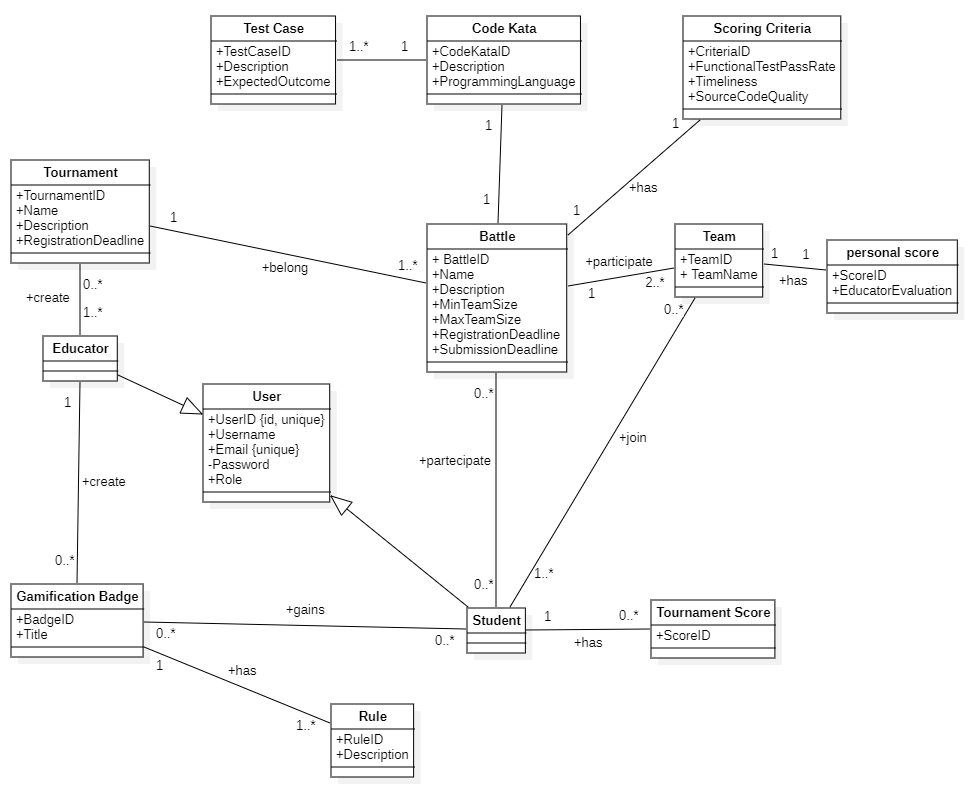
\includegraphics[scale=0.6]{DCD.png}
    \caption{Domain Class Diagram}
    \label{fig:DCD}
\end{figure}


\subsubsection{Statecharts}
Two state charts are discussed in this section which are fundamental for understanding the life cycle of a tournament and the process to join a battle. \\

\begin{figure}[H]
    \centering
    \textbf{Tournament life cycle} \\
    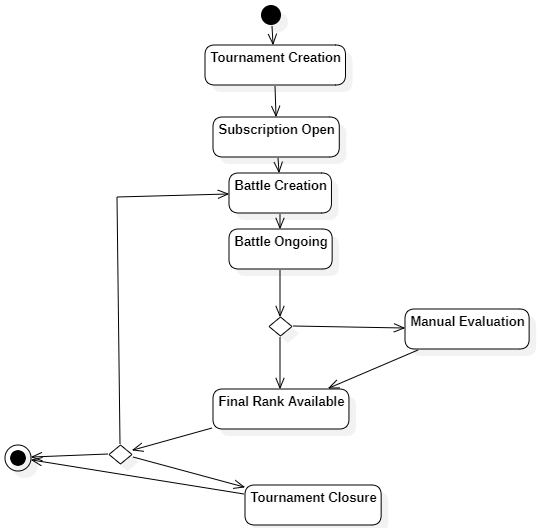
\includegraphics[scale=0.65]{Tournament.png}
\end{figure}
\noindent
The first state is \textit{Tournament Creation}, in this state the educator creates the tournament and invites collaborators;
Once done, the tournament goes in the \textit{Subscription Open} state waiting for students to join the tournament. \\
After the registration deadline, educators can create battles for the students who joined the tournament in the \textit{Battle Creation} state. \\
Students who successfully joined the battle can now compete by sending their solution before the deadline in the \textit{Battle Ongoing} state; Their solution will be automatically evaluated every time they are submitted and after the end of the battle, if required, a \textit{Manual Evaluation} is performed by the educator. \\
After the evaluation step, the \textit{Final Rank Available} state is reached and educators can then decide whether to create new battles(and return to the \textit{Battle Creation} state) or close the tournament reaching the final \textit{Tournament Closure} state. \\

\begin{figure}[H]
    \centering
    \textbf{Battle life cycle} \\
    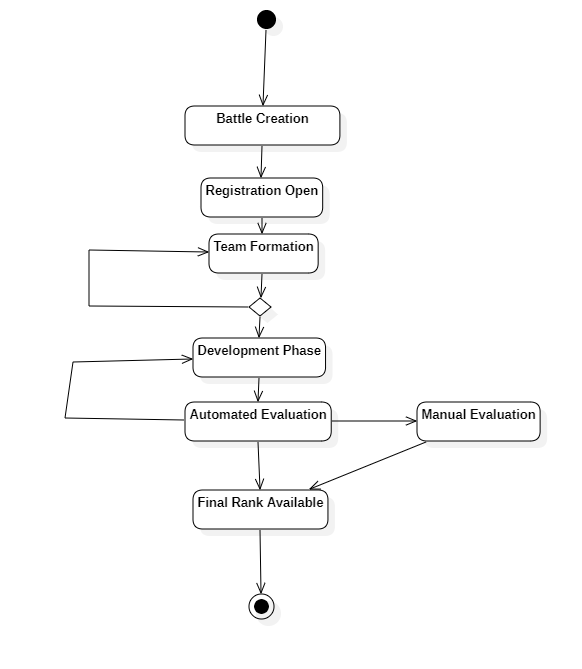
\includegraphics[scale=0.65]{Battle.png}
\end{figure}
\noindent
The first state is \textit{Battle Creation}: in this state, the battle is being created by the Educator, who sets the available programming language(s), the minimum and maximum team size, the time slots for subscribing and submitting the solution, and eventually enables the manual evaluation, then proceeds to upload the files about the problem.\\
Then, when the battle has been successfully created, the \textit{Registration Open} event is reached: after the registrations have opened students can proceed to start the \textit{Team Formation}, inviting others who are participating in the tournament in their team for the battle.\\
When the deadline for subscription ends the battle starts: every team starts its \textit{Development Phase}, during which students work to find a solution to the problem of the battle.\\
Every time a solution is submitted the system performs an \textit{Automated Evaluation} on it to give it a score, which is immediately visible in the provisional rank of the battle.\\
When the deadline for solution submission expires, a\textit{Manual Evaluation}, if previously enabled while creating the battle, is performed by the Educator on all the submitted solutions.\\
After that, the battle has ended, and it reaches the \textit{final Rank Available} state: the final results are visible and the tournament general rank is updated.\\
\subsection{Product Functions}

\subsubsection{Sign Up and Login}
These functions will be available to all the users: during the sign-up procedure everyone has to insert an e-mail and a password: these will be also the credentials to log in to the account that is being created.\\
The inserted e-mail will be verified from the system with a confirmation e-mail sent to the user.\\
Once this step is done the user will have to insert their personal data: Name, Surname, a username that will be the one who will be seen by the other users, and the type of user (Educator or Student).
\subsubsection{Tournament creation}
Each Educator can use the system to create tournaments for Students, that will compete singularly in them.
When creating a tournament an Educator has to set the list of available programming languages, the number of battles and to give it a name, they can in addition choose to set it as private protecting it with an alphanumerical access key.\\
The tournaments can also be handled by more than one Educator: collaborators can be added from the creation page, and they can create battles and manually evaluate the solutions provided by the Students if needed, but they cannot create badges.
Once an Educator has created a tournament every user in the system is notified and can join it.
The creator has to set a subscription deadline: as the deadline expires the tournament status passes from opened to ongoing and no one can join it anymore.
\subsubsection{Tournament subscription}
Each student can subscribe to a tournament: once they have found a tournament in which they want to compete, exploring the list or searching it there by name or creator, they can click and join it, inserting the access key if it's required.
\subsubsection{Battle creation}
In the context of an ongoing tournament Educators have to set the options of each battle before making it start: they have to choose the maximum team size in that battle, the language(s) for that specific battle picked from the tournament's ones, and to set the subscription and solution submission deadline.
He has also to decide if the solutions will be evaluated totally by the system or if he also wants to manually check the solutions at the end of the battle.
After having done that the Educator has to upload the text and test cases for the problem that the Students have to solve in that battle: when the Educator confirms the creation of a battle a repository containing the uploaded files will be created on GitHub; it will be made available to all Students involved in the battle when the deadline expires.
Once all this has been done the Educator confirms the creation of the battle: all the Students that are subscribed to the tournament are notified and the timer for the registration starts.
\subsubsection{Battle joining}
Each student subscribed to a tournament can join its battles: they receive a notification every time a new battle is ready to start and they have time to join it until the deadline set by the Educator has expired.\\
As the deadline for subscribing expires each competing student will be allowed to see the link of the repository where they will find the text of the exercise and the test cases that the educator uploaded: each team has to fork the repository and paste the link of his copy in an apposite form in the app so that the System can visit the repository and check the solutions when it's needed.
\subsubsection{Code Evaluation}
The System, during a battle, will use CodeScene, a tool for Code Static Analysis, to give a score to each competitor: the score is assigned each time a solution is pushed on the GitHub repository so that a live provisional rank is always visible for all the duration of the battle to all the Students involved. 
When the battle ends, and after the eventual manual evaluation by the Educator, Students will be able to see the final scores of all the competitors in the rank of the battle, and also the updated tournament rank.\\
The score is a number from 0 to 100, determined based on criteria like correctness but also time and space efficiency and so on.
If the manual evaluation is disabled for the battle the score will be entirely assigned by the System, otherwise, it will assign at maximum only a part of the available 100 points, to which it will be summed the other part of the score that will be assigned from the Educator.
\subsubsection{Gamification Badges}
Educators are allowed, in the context of a tournament, to create Gamification Badges: they can be only added by an educator when he is creating a tournament, neither he nor the eventual collaborator can modify them or add other ones any later .\\
Badges are achievements that the Students can gain by satisfying a requirement.\\
When creating a badge, an educator has to give it a name, optionally an image, and to write a brief description of the requirement: these are the things that students will be able to see.\\
To make the system be able to analyze the requirement and eventually assign the badge when it's necessary, the Educator has also to write it as a boolean condition built on variables given by the System.\\
The variables represent the most important stats regarding battles and tournaments, and they are related to many aspects:\\
\begin{itemize}
    \item \textbf{Score}: there is a variable related to the tournament and battle score of a single student 
    \item \textbf{Commits}: there are variables related to team commit number and to the maximum number of commits made by a team in a battle.\\
    There are also the same variables regarding single students in the context of the whole tournament.
    \item \textbf{Code}: there are variables about the code correctness, the execution speed for every single team and two variables representing the fastest working code in the battle and the first team to submit a correct solution to the problem.
    \item \textbf{Rank}: there are variables representing the rank position of each student in a battle 
    or in the total rank of the tournament.
\end{itemize}
If a parameter value changes the system verifies the conditions that have been created and, if someone has satisfied it, gives him the badge and sends him a notification.
\subsubsection{Stats and Rankings}
Each user is allowed to explore other accounts: in particular, the tournament ranks (ended and ongoing ones) and the badges of a user are public; everyone can see them clicking on their account.

\subsection{User Characteristics}
The system is designed to interact with the following two different kinds of users:
\subsubsection{Educator}
An educator is a user who registers through the CKB app by creating an "educator account", it can create tournaments and battles, invite collaborators to the tournament, evaluate the solutions provided by the students, and create badges for each tournament (optional).
\subsubsection{Student}
A student is a user who registered through the CKB app by creating a "student account", it can join tournaments and battles, invite other students in their current team, and submit solutions for the battles in which it joined.
\subsection{Assumptions, dependencies and constraints}

\subsubsection{Regulatory Polices}
The CKB application will ask for user's personal information like name, surname, and email address. Email addresses won’t be used for commercial purposes. Personal information will be processed in compliance with the GDPR.

\subsubsection{Domain Assumptions}
The following are the domain assumptions that need to be satisfied for the correct behavior of CKB. Since those situations are out of the control of the system, they are taken for granted.\\\\
$[D1]$ User must have an internet connection.\\
$[D2]$ User must have a GitHub account.\\
$[D3]$ User must know how to use GitHub properly (push, pull, branch, etc.).\\
$[D4]$ Connection between systems must be reliable.\\
$[D5]$ Test cases provided by educators must be correct.\\
$[D6]$ GitHub works as expected.\\
$[D7]$ The static Analysis tool works reliably.\\

\section{Specific Requirements}
\subsection{External Interface Requirements}
\subsubsection{User Interfaces}
This section presents the user interface through which both students and educators can:
\begin{itemize}
    \item Log in
    \item Sign Up
    \item Access personal dashboard
\end{itemize}
The needs of educators and students are not the same, therefore they are going to get access to different views:\\
Educators have access to specific views that allow them to handle tournaments and battles while students must be able to join tournaments and battles, as well as invite members in their group.



\begin{figure}[H]
    \centering
    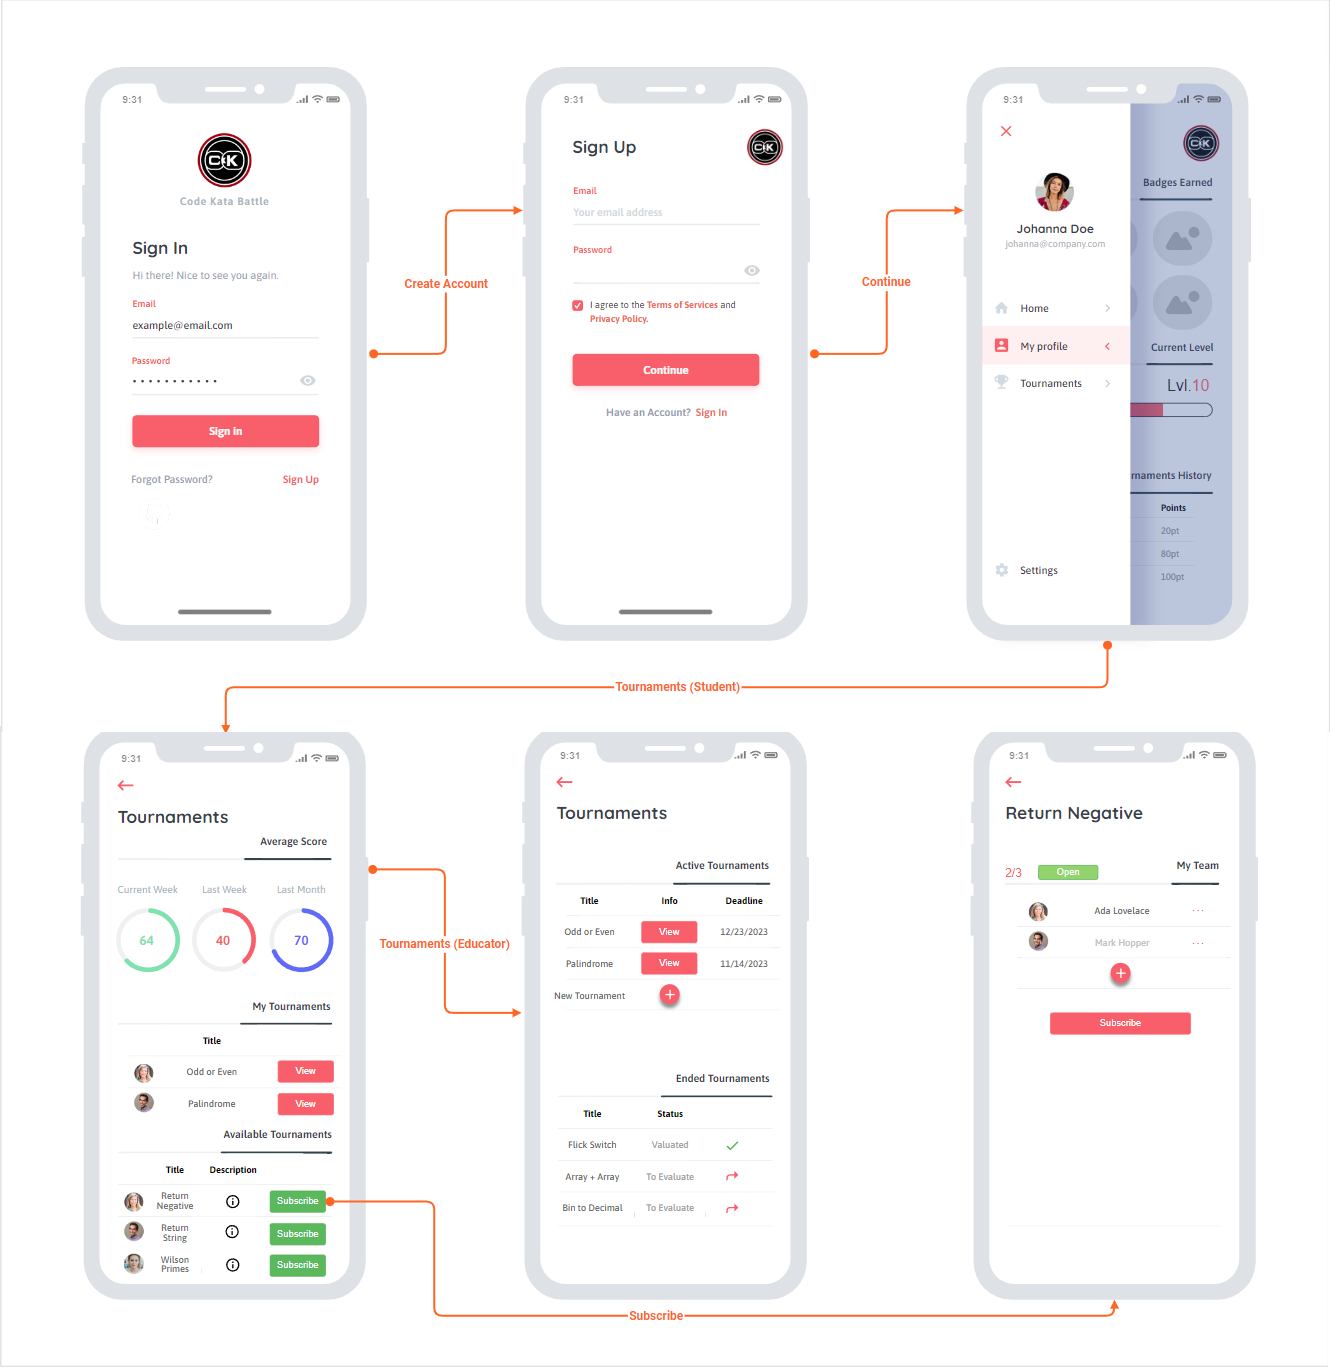
\includegraphics[width=\linewidth]{Mobile UI.png}
    \caption{Mobile User Interface}
\end{figure}

\begin{figure}
    \centering
    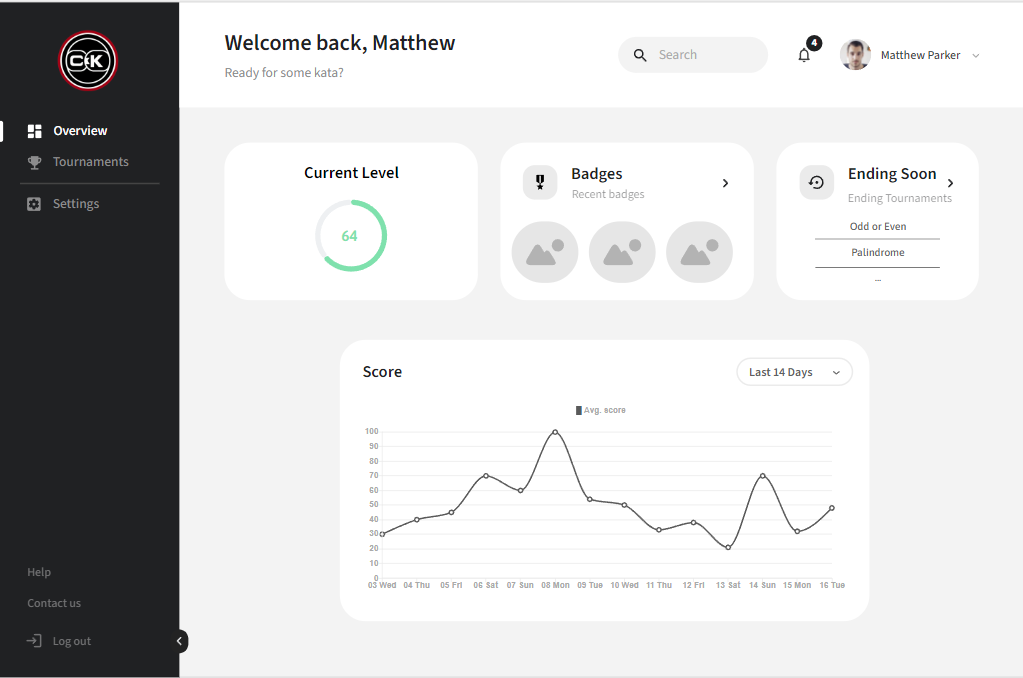
\includegraphics[width=\linewidth]{Web UI.png}
    \caption{Web User Interface}
\end{figure}

\begin{figure}
    \centering
    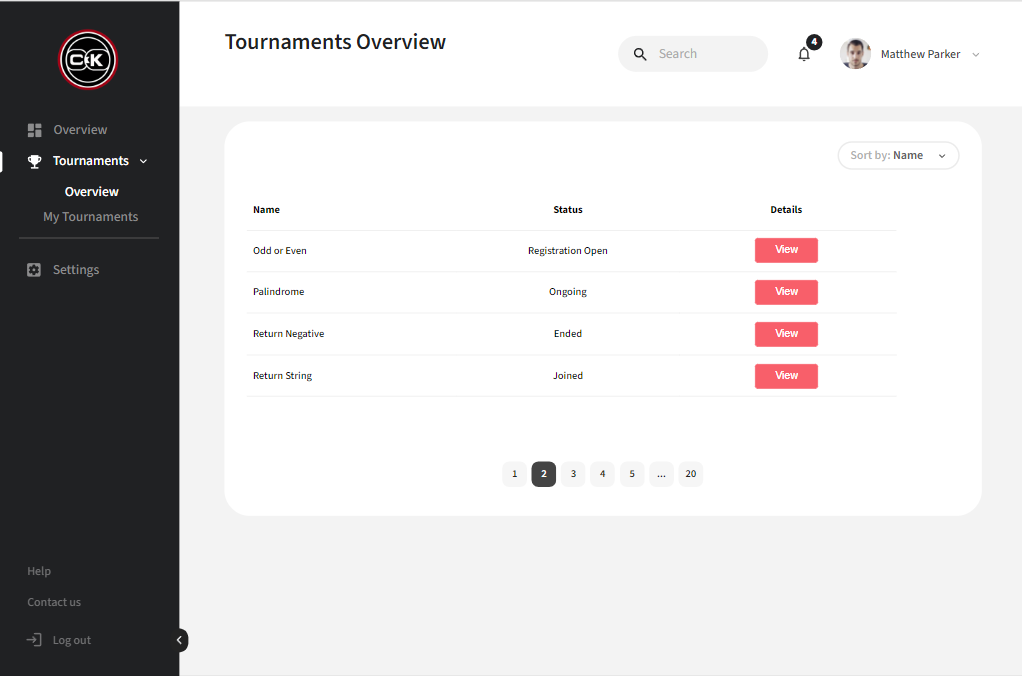
\includegraphics[width=\linewidth]{Web UI 2.png}
    \caption{Web Interface Student}
\end{figure}

\begin{figure}
    \centering
    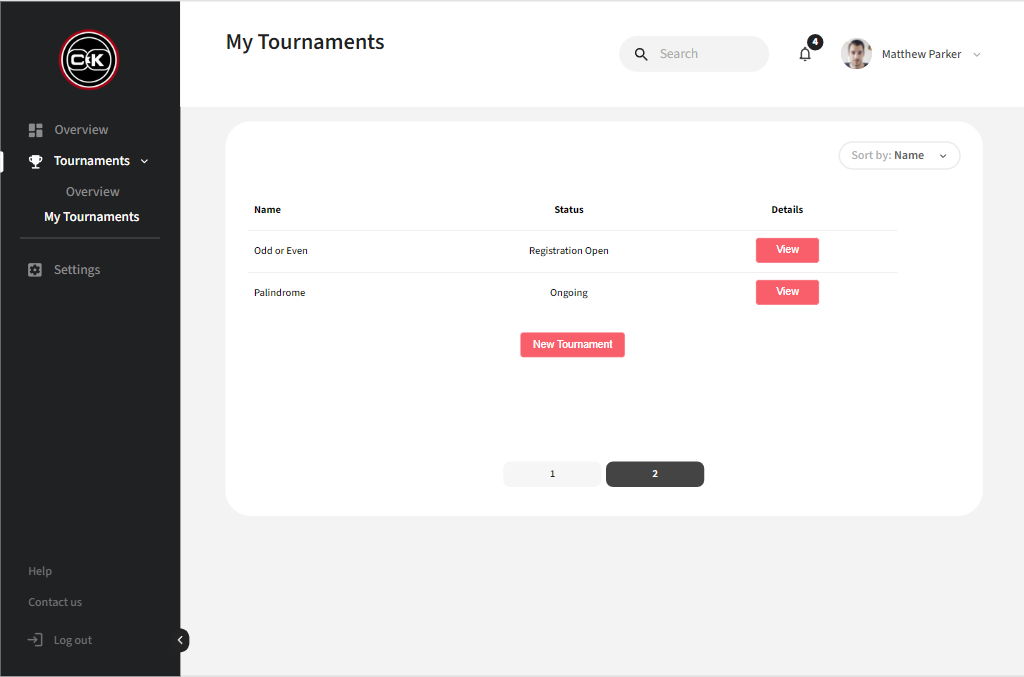
\includegraphics[width=\linewidth]{Web UI 3.png}
    \caption{Web Interface Educator}
\end{figure}
\newpage
\subsubsection{Hardware Interfaces}

The system offers to the users different services (see paragraph \textbf{2.2}) that can be accessed by any device with an internet connection whether it's through the app or web app.
                            
\subsubsection{Software Interfaces}
The system relies on different software interfaces, more specifically:
\begin{itemize}
    \item \textbf{GitHub API:} The system uses this API to create the repository of the battle, moreover, can receive notifications from GitHub every time a new solution to the problem has been uploaded by a student.
    \item \textbf{CodeScene API:} The system uses this API to evaluate all the solutions uploaded by students: every time a new solution is uploaded, the system sends it to CodeScene for evaluation and then, converts the result into an integer number.
\end{itemize}

\subsubsection{Communication Interfaces}
The System uses an Internet connection to communicate with GitHub and all the users: it should have a uniform interface so that the communication is always reliable.


\subsection{Functional Requirements}
$[FR1]$ The system allows Users to sign up.\\
$[FR2]$ The system allows Users to log in.\\
$[FR3]$ The system allows Educators to create tournaments.\\
$[FR4]$ The system allows Educators to set a deadline for subscribing to the tournament.\\
$[FR5]$ The System allows Educators to set a list of programming languages that will be used in the tournament.\\
$[FR6]$ The system allows Educators to invite other Educators as collaborators for a tournament\\
$[FR7]$ The system allows Educators to set the number of battles in a tournament.\\
$[FR8]$ The system allows Educators to create battles.\\
$[FR9]$ The system allows Educators to set a deadline for the subscription to the battle.\\
$[FR10$ The system allows Educators to set a deadline for the submission of the solutions to the battle.\\
$[FR11]$ The System allows educators to choose which of the languages of the tournament will be used in each battle.\\
$[FR12]$ The System allows Educators to upload the files with the text of the problem and test cases for the battle\\
$[FR13]$ The system allows Educators to set the maximum number of students per team in a battle.\\
$[FR14]$ The system allows Educators to choose whether and when the scores will be assigned in a totally automatic way or also through a manual verification by themselves\\
$[FR15]$ The system allows Educators to create badges for a specific tournament.\\
$[FR16]$ The system allows Educators to build the requirements for achieving a badge.\\
$[FR17]$ The system allows Students to see what are the active badges in a tournament and what they have to do to achieve them.\\
$[FR18]$ The system allows Students to join a tournament.\\
$[FR19]$ The system allows Students to invite other students to form teams for a battle\\
$[FR20]$ The system allows Students to join a battle. \\
$[FR21]$ The system allows Students to know about the provisional scores of all students, updated for every solution submitted, for all the duration of a battle\\
$[FR22]$ The system allows Educators to see the list of the active tournaments they have created.\\
$[FR23]$ The system allows Students to see the list of the active tournaments they have joined.\\
$[FR24]$ The system allows Users to see the stats of any other account registered in the system\\
$[FR25]$ The system allows Users to search for other accounts or tournaments on the search bar\\


\subsubsection{Use Case Diagrams}

\begin{figure}[H]
  \centering
  \textbf{Student Use Case Diagram} \\
  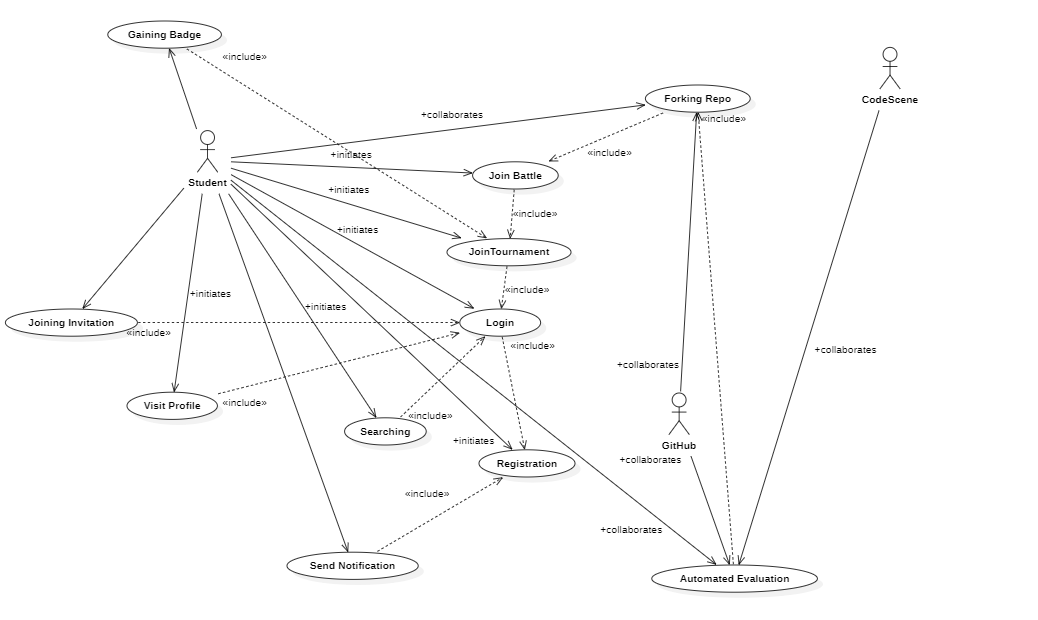
\includegraphics[width=1.2\linewidth]{UCStudent.png}
\end{figure}

\begin{figure}[H]
  \centering
  \textbf{Educator Use Case Diagram} \\
  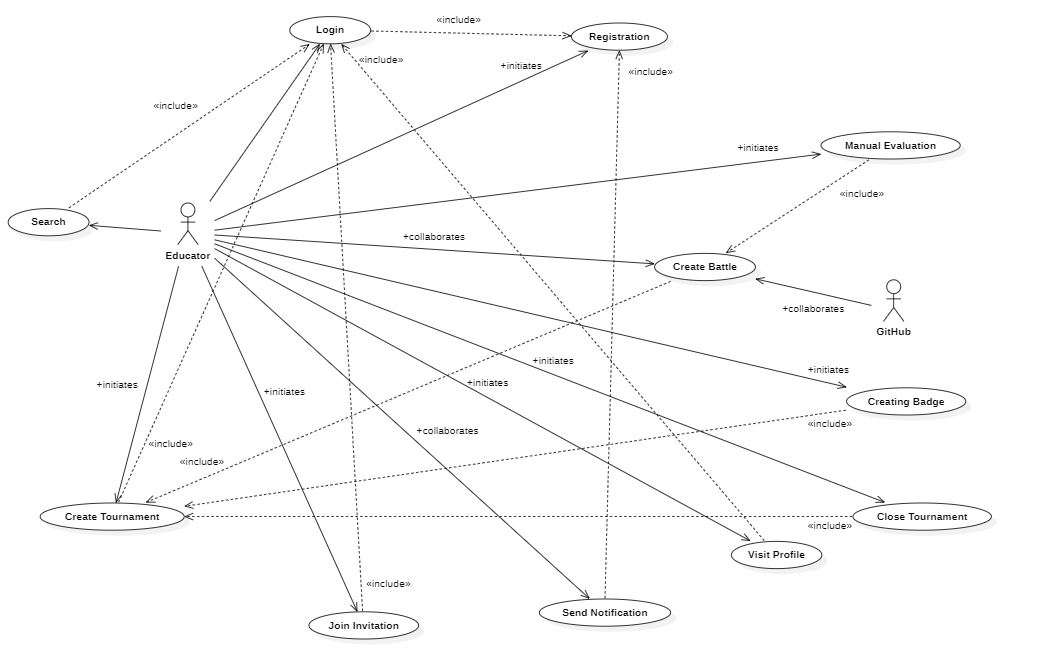
\includegraphics[width=1.1\linewidth]{UCEducator.png}
\end{figure}

\newpage

\subsubsection{Use Cases}
The following are the use cases that can happen within the system:
\begin{table}[H]
 \renewcommand{\arraystretch}{1.5}
    \centering
    \raggedright\textbf{[UC1] Registration }
    \begin{tabular}{|l|p{10cm}|}
        \hline
        \textbf{Name} & Registration \\
        \hline
        \textbf{Actor} & User \\
        \hline
        \textbf{Entry Condition} & 
        The user has opened the application \\
        \hline
        \textbf{Event Flow} & 
        \begin{enumerate}[align=left, topsep=0pt, partopsep=0pt]
            \item The user opens the application 
            \item The user clicks on the button” Sign Up” 
            \item The system shows the registration form 
            \item The user inserts his email and a password 
            \item The system sends a confirmation email to the user through an email provider 
            \item The user confirms his email by clicking on the link received by email 
            \item The system shows a form asking for personal information, including the type of account the user wants to create (Student or Educator)
            \item The user inserts the requested data 
        \end{enumerate} \\
        \hline
        \textbf{Exit Condition} & Registration has been successful. The user’s data is stored in the system’s database. The user then will be able to log into the system by using their credentials.  \\
        \hline
        \textbf{Exception} & The user is already registered to the system. The system will send a notification message telling the user that there is an account with that email. \\
        \hline
    \end{tabular}
\end{table}


\begin{table}
 \renewcommand{\arraystretch}{1.5}
    \centering
    \raggedright\textbf{[UC2] User Login}
    \begin{tabular}{|l|p{10cm}|}
        \hline
        \textbf{Name} & User Login \\
        \hline
        \textbf{Actor} & User \\
        \hline
        \textbf{Entry Condition} & 
        The user has opened the application\\
        \hline
        \textbf{Event Flow} & 
        \begin{enumerate}[align=left, topsep=0pt, partopsep=0pt]
            \item The user inserts his username and password in the form
            \item The user clicks on the “Login” button
            \item The system checks the credentials
            \item The application shows the dashboard
        \end{enumerate} \\
        \hline
        \textbf{Exit Condition} & The user has access to the services  \\
        \hline
        \textbf{Exception} & The data inserted is not valid. The system returns to the entry condition. \\
        \hline
    \end{tabular}
\end{table}

\begin{table}
 \renewcommand{\arraystretch}{1.5}
    \centering
    \raggedright\textbf{[UC3] Create Tournament}
    \begin{tabular}{|l|p{10cm}|}
        \hline
        \textbf{Name} & Create Tournament \\
        \hline
        \textbf{Actor} & Educator \\
        \hline
        \textbf{Entry Condition} & The educator is logged into the platform \\
        \hline
        \textbf{Event Flow} & 
        \begin{enumerate}[align=left, topsep=0pt, partopsep=0pt]
            \item The educator clicks on the button to create a tournament
            \item The educator puts information about the tournament 
            \item The educator creates badges \textbf{[UC7]}
            \item The educator invites other educators to join the tournament as collaborators
            \item The educator clicks on the “Confirm Creation” button
            \item The application shows the tournament environment 
        \end{enumerate} \\
        \hline
        \textbf{Exit Condition} & The educator successfully created the tournament  \\
        \hline
    \end{tabular}
\end{table}

\begin{table}
 \renewcommand{\arraystretch}{1.5}
    \centering
    \raggedright\textbf{[UC4] Create Battle}
    \begin{tabular}{|l|p{10cm}|}
        \hline
        \textbf{Name} & Battle\\
        \hline
        \textbf{Actor} & Educator, GitHub \\
        \hline
        \textbf{Entry Condition} & The educators logged into the platform and selected the tournament in which they wanted to create a battle \\
        \hline
        \textbf{Event Flow} & 
        \begin{enumerate}[align=left, topsep=0pt, partopsep=0pt]
            \item The educator clicks on “create battle” button
            \item The educator specifies information about the battle (name, text information, subscription deadline, submission deadline, etc…)
            \item The educator uploads the track of the problem and the test cases 
            \item The educator clicks on the “confirm creation” button
            \item The system creates the repo with the uploaded files
            \item The system sends a notification to users about the creation of the battle \textbf{[UC9]}
        \end{enumerate} \\
        \hline
        \textbf{Exit Condition} & The educator successfully created the battle  \\
        \hline
    \end{tabular}
\end{table}

\begin{table}
 \renewcommand{\arraystretch}{1.5}
    \centering
    \raggedright\textbf{[UC5] Join Battle}
    \begin{tabular}{|l|p{10cm}|}
        \hline
        \textbf{Name} & Join Battle \\
        \hline
        \textbf{Actor} & Student, GitHub \\
        \hline
        \textbf{Entry Condition} & User logged into the application and is on the battle page;
        The battle is open for registration \\
        \hline
        \textbf{Event Flow} & 
        \begin{enumerate}[align=left, topsep=0pt, partopsep=0pt]
             \item The student clicks on the “join battle” button
             \item The student sees all the information about the battle 
             \item The student sends the invitations to other students and waits for acceptances/rejections to form their team
             \item Students click on “Confirm”
         \end{enumerate} \\
        \hline
        \textbf{Exit Condition} & Student/Team successfully joined the battle \\
        \hline
    \end{tabular}
\end{table}

\begin{table}
 \renewcommand{\arraystretch}{1.5}
    \centering
    \raggedright\textbf{[UC6] Student Joins Tournament}
    \begin{tabular}{|l|p{10cm}|}
        \hline
        \textbf{Name} & Student Joins Tournament \\
        \hline
        \textbf{Actor} & Student \\
        \hline
        \textbf{Entry Condition} & 
        User logged into the application and is on the tournament page; The tournament is open for registration  \\
        \hline
        \textbf{Event Flow} & 
        \begin{enumerate}[align=left, topsep=0pt, partopsep=0pt]
            \item The student clicks on the “Join Tournament” button 
            \item The student sees all the information about the tournament
            \item The student clicks on the “Confirm Joining” button
        \end{enumerate} \\
        \hline
        \textbf{Exit Condition} & The student joined the tournament successfully  \\
        \hline
    \end{tabular}
\end{table}

\begin{table}
 \renewcommand{\arraystretch}{1.5}
    \centering
    \raggedright\textbf{[UC7] Create Badge}
    \begin{tabular}{|l|p{10cm}|}
        \hline
        \textbf{Name} & Badge Creation \\
        \hline
        \textbf{Actor} & Educator \\
        \hline
        \textbf{Entry Condition} & The educators logged into the platform and started the creation of the tournament  \\
        \hline
        \textbf{Event Flow} & 
        \begin{enumerate}[align=left, topsep=0pt, partopsep=0pt]
            \item The educator clicks on the “Create Badge” button
            \item The educator chooses a title for the badge
            \item The educator uploads an image for the badge
            \item The educator writes the description of requirements for the badge
            \item The educator builds the conditions with variables for the badge 
            \item The educator clicks on the “confirm badge” button
        \end{enumerate} \\
        \hline
        \textbf{Exit Condition} & The educator successfully created a badge \\
        \hline
        \textbf{Exception} & The educator didn't build the conditions in step \textbf{5} correctly  \\
        \hline
    \end{tabular}
\end{table}

\begin{table}
 \renewcommand{\arraystretch}{1.5}
    \centering
    \raggedright\textbf{[UC8] Assigning Badge}
    \begin{tabular}{|l|p{10cm}|}
        \hline
        \textbf{Name} & Assigning Badge \\
        \hline
        \textbf{Actor} & Student \\
        \hline
        \textbf{Entry Condition} & The educators have defined badges with associated rules and criteria; A battle or the tournament has ended\\
        \hline
        \textbf{Event Flow} & 
        \begin{enumerate}[align=left, topsep=0pt, partopsep=0pt]
            \item The system verifies the fulfillment of conditions for achieving a badge
            \item The system eventually awards the badge to the Student
        \end{enumerate} \\
        \hline
        \textbf{Exit Condition} & The student receives the badge \\
        \hline
    \end{tabular}
\end{table}

\begin{table}
 \renewcommand{\arraystretch}{1.5}
    \centering
    \raggedright\textbf{[UC9] Notify Participants}
    \begin{tabular}{|l|p{10cm}|}
        \hline
        \textbf{Name} & Notification System \\
        \hline
        \textbf{Actor} & User \\
        \hline
        \textbf{Entry Condition} & A significant event occurs within the CKB platform\\
        \hline
        \textbf{Event Flow} & 
        \begin{enumerate}[align=left, topsep=0pt, partopsep=0pt]
            \item The system identifies a significant event
            \item The system chooses the nature of the event
            \item The system chooses the Users to whom the notification will be sent
            \item The system generates notifications containing relevant information
            \item The system sends out notifications
        \end{enumerate} \\
        \hline
        \textbf{Exit Condition} & User receive the notification successfully \\
        \hline
    \end{tabular}
\end{table}

\begin{table}
 \renewcommand{\arraystretch}{1.5}
    \centering
    \raggedright\textbf{[UC10] Automated Evaluation}
    \begin{tabular}{|l|p{10cm}|}
        \hline
        \textbf{Name} & Automated Evaluation \\
        \hline
        \textbf{Actor} & Static Analysis Tool \\
        \hline
        \textbf{Entry Condition} & The student/team pushes a new commit to the main branch of their forked repository containing their code solution\\
        \hline
        \textbf{Event Flow} & 
        \begin{enumerate}[align=left, topsep=0pt, partopsep=0pt]
            \item The CKB platform retrieves the latest source code from the Student/Team's repository related to the specific battle
            \item The system sends code and test cases to the Static Analysis Tool 
            \item The Static Analysis Tool analyzes the code 
            \item The Static Analysis Tool sends back the results to the System
            \item The system calculates a score
            \item The system updates the battle score of the respective Team
            \item The system notifies participants \textbf{[UC9]}
        \end{enumerate} \\
        \hline
        \textbf{Exit Condition} & The battle score is updated \\
        \hline
    \end{tabular}
\end{table}

\begin{table}
 \renewcommand{\arraystretch}{1.5}
    \centering
    \raggedright\textbf{[UC11] Manual Evaluation}
    \begin{tabular}{|l|p{10cm}|}
        \hline
        \textbf{Name} & Manual Evaluation \\
        \hline
        \textbf{Actor} & Educator \\
        \hline
        \textbf{Entry Condition} & The battle has ended and the solutions have been submitted, manual evaluation enabled\\
        \hline
        \textbf{Event Flow} & 
        \begin{enumerate}[align=left, topsep=0pt, partopsep=0pt]
            \item The educator accesses the battle page
            \item The educator selects the link of a solution he wants to evaluate
            \item The educator evaluates the solution 
            \item The educator inserts the score in the system (the sum of the maximum score assignable by the system and the one assignable by the Educator is 100)
            \item The educator confirms the inserted scores
        \end{enumerate} \\
        \hline
        \textbf{Exit Condition} & Final marks are calculated and published by the system  \\
        \hline
        \textbf{Exception} & 
        \begin{itemize}[topsep=0pt, partopsep=0pt]
            \item Invalid score assigned by the educator
            \item Confirmation while one or more scores are missing
        \end{itemize} \\
        \hline
    \end{tabular}
\end{table}

\begin{table}
 \renewcommand{\arraystretch}{1.5}
    \centering
    \raggedright\textbf{[UC12] Creating Repository Fork}
    \begin{tabular}{|l|p{10cm}|}
        \hline
        \textbf{Name} & Creating Fork \\
        \hline
        \textbf{Actor} & Student, GitHub \\
        \hline
        \textbf{Entry Condition} & Subscription deadline for the battle has expired\\
        \hline
        \textbf{Event Flow} & 
        \begin{enumerate}[align=left, topsep=0pt, partopsep=0pt]
            \item The student accesses the battle page
            \item The system shows the User the link to the GitHub main repository for the battle
            \item The student creates a branch for the repository  
            \item The student sends the link of the branch to the system
            \item The student clicks on “confirm”
            \item The system checks that the link is valid
        \end{enumerate} \\
        \hline
        \textbf{Exit Condition} & Student/team successfully registered their branch \\
        \hline
        \textbf{Exception} & Invalid link \\
        \hline
    \end{tabular}
\end{table}

\begin{table}
 \renewcommand{\arraystretch}{1.5}
    \centering
    \raggedright\textbf{[UC13] Close Tournament}
    \begin{tabular}{|l|p{10cm}|}
        \hline
        \textbf{Name} & Tournament Closure \\
        \hline
        \textbf{Actor} & Educator \\
        \hline
        \textbf{Entry Condition} & All battles have ended\\
        \hline
        \textbf{Event Flow} & 
        \begin{enumerate}[align=left, topsep=0pt, partopsep=0pt]
            \item The educator clicks on “Close Tournament”
            \item Students are notified that the tournament has ended \textbf{[UC9]}
            \item The system shows the final results on the tournament homepage 
        \end{enumerate} \\
        \hline
        \textbf{Exit Condition} & The tournament is closed \\
        \hline
        \textbf{Exception} & Ongoing battle \\
        \hline
    \end{tabular}
\end{table}

\begin{table}
 \renewcommand{\arraystretch}{1.5}
    \centering
    \raggedright\textbf{[UC14] Visit Profile}
    \begin{tabular}{|l|p{10cm}|}
        \hline
        \textbf{Name} & Visit Profile \\
        \hline
        \textbf{Actor} & User \\
        \hline
        \textbf{Entry Condition} & User has logged into the system\\
        \hline
        \textbf{Event Flow} & 
        \begin{enumerate}[align=left, topsep=0pt, partopsep=0pt]
            \item The user clicks on an account or searches it \textbf{[UC16]}
            \item The system shows the account information to the user
        \end{enumerate} \\
        \hline
        \textbf{Exit Condition} & The user can see the requested profile \\
        \hline
    \end{tabular}
\end{table}

\begin{table}
 \renewcommand{\arraystretch}{1.5}
    \centering
    \raggedright\textbf{[UC15] Joining Invitation}
    \begin{tabular}{|l|p{10cm}|}
        \hline
        \textbf{Name} & Joining Invitation \\
        \hline
        \textbf{Actor} & User \\
        \hline
        \textbf{Entry Condition} & A user has received an invitation notification and has logged into the system\\
        \hline
        \textbf{Event Flow} & 
        \begin{enumerate}[align=left, topsep=0pt, partopsep=0pt]
            \item The user accesses the notifications section
            \item The user clicks on the notification
            \item The system shows the information about the invitation
            \item The user accepts or declines the invitation
        \end{enumerate} \\
        \hline
        \textbf{Exit Condition} & The invitation has been accepted or declined \\
        \hline
        \textbf{Exception} & The invitation has been retired \\
        \hline
    \end{tabular}
\end{table}

\begin{table}
 \renewcommand{\arraystretch}{1.5}
    \centering
    \raggedright\textbf{[UC16] Searching}
    \begin{tabular}{|l|p{10cm}|}
        \hline
        \textbf{Name} & Searching \\
        \hline
        \textbf{Actor} & User \\
        \hline
        \textbf{Entry Condition} & User has logged into the system \\
        \hline
        \textbf{Event Flow} & 
        \begin{enumerate}[align=left, topsep=0pt, partopsep=0pt]
            \item The user clicks on the search bar 
            \item The user digits a keyword
            \item The system shows the results of the research
        \end{enumerate} \\
        \hline
        \textbf{Exit Condition} & The user can see the result of his research \\
        \hline
    \end{tabular}
\end{table}


\subsubsection{Sequence Diagrams}

\begin{figure}[H]
  \centering
  \textbf{[UC1] Registration} \\
  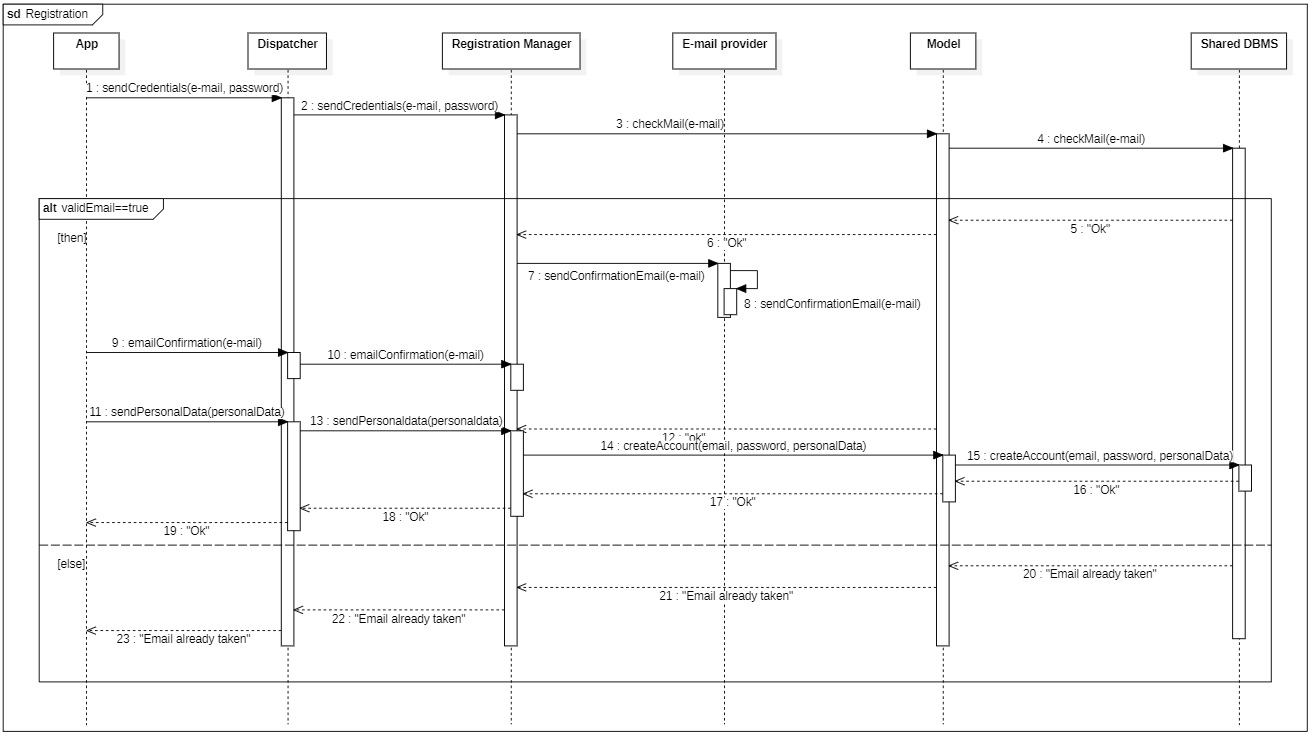
\includegraphics[width=\linewidth]{UC1.png}
\end{figure}

\begin{figure}[H]
  \centering
  \textbf{[UC2] Login} \\
  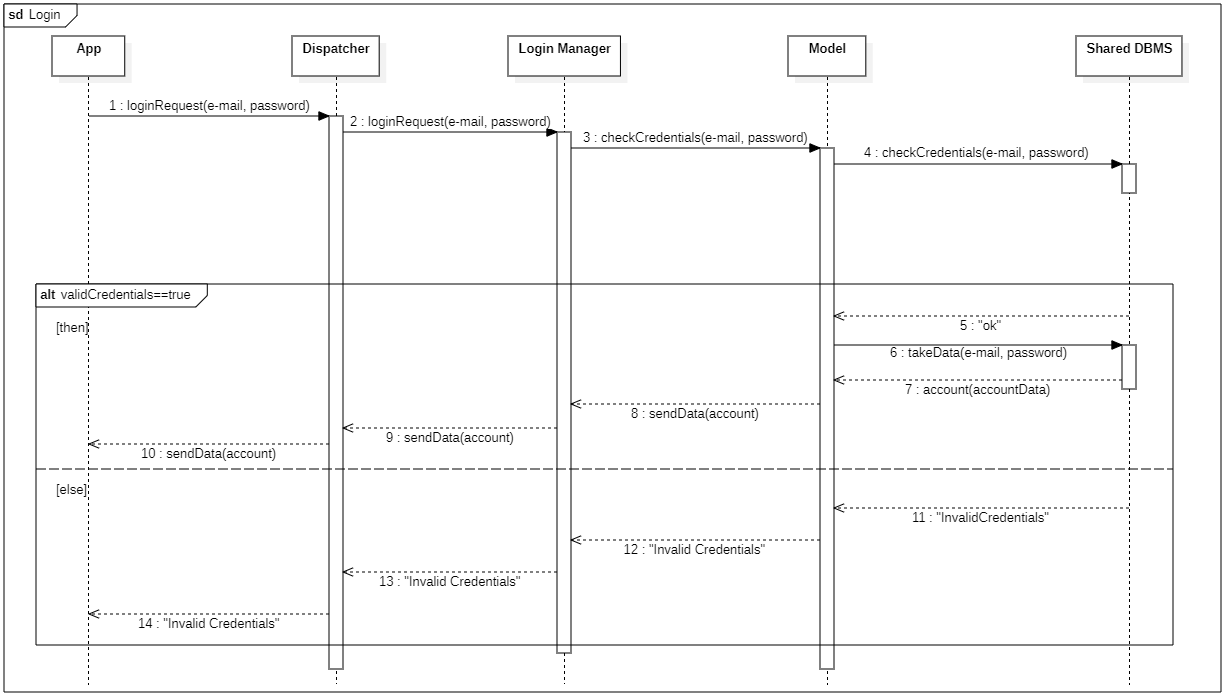
\includegraphics[width=\linewidth]{UC2.png}
\end{figure}

\begin{figure}[H]
  \centering
  \textbf{[UC3] Create Tournament} \\
  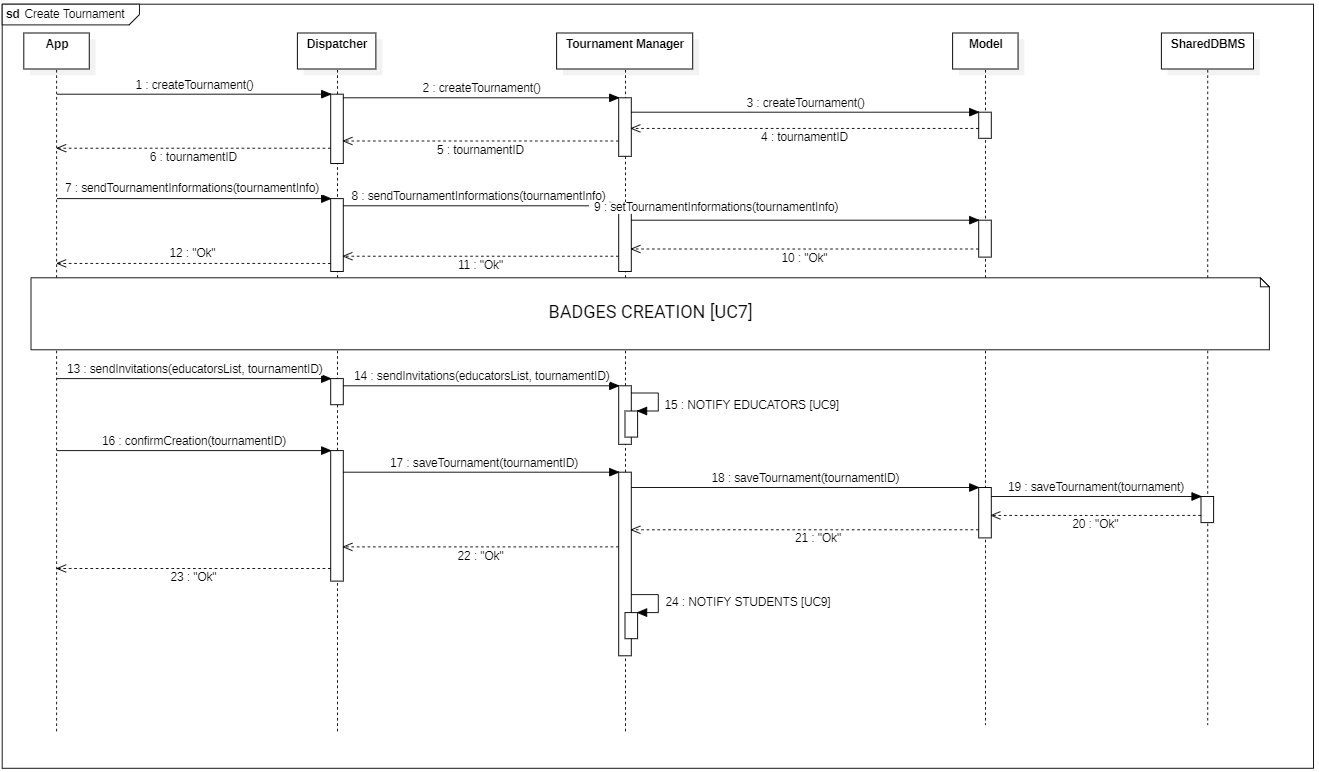
\includegraphics[width=\linewidth]{UC3.png}
\end{figure}

\begin{figure}[H]
  \centering
  \textbf{[UC4] Create Battle} \\
  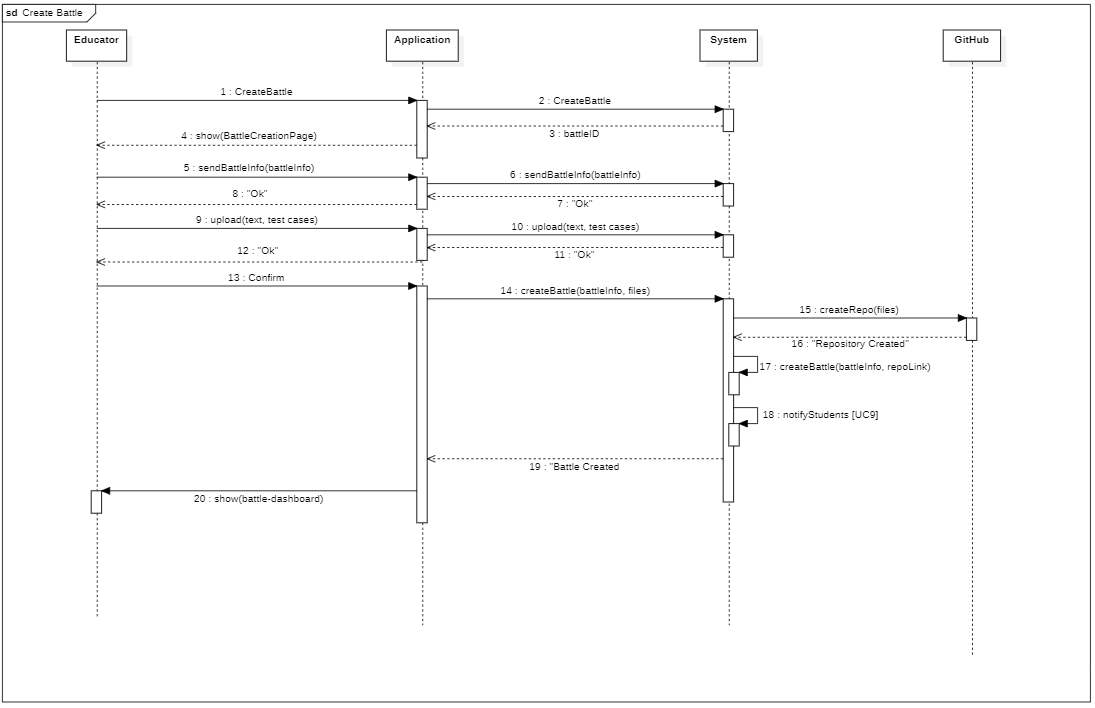
\includegraphics[width=\linewidth]{UC4.png}
\end{figure}

\begin{figure}[H]
  \centering
  \textbf{[UC5] Join Battle} \\
  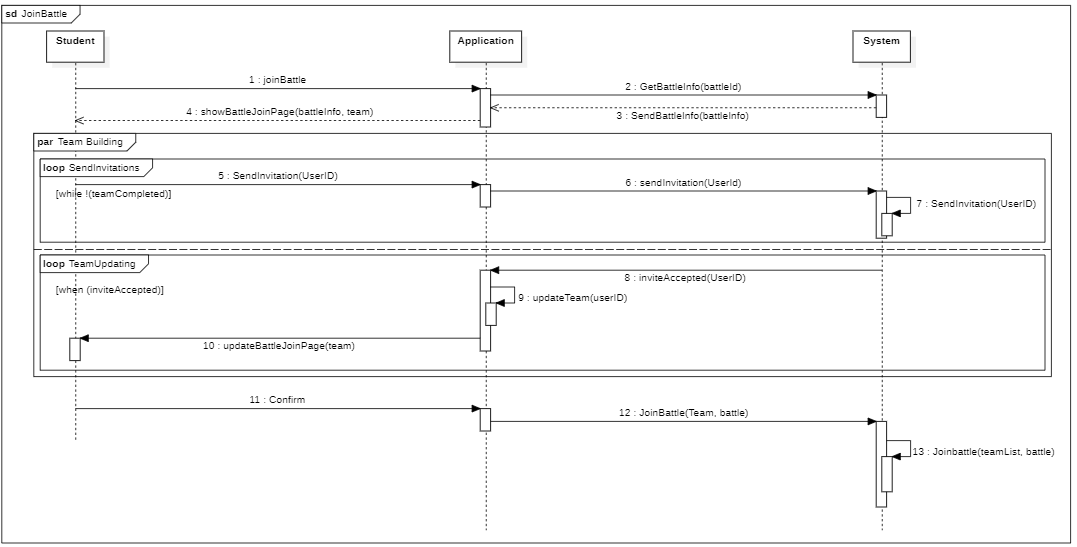
\includegraphics[width=\linewidth]{UC5.png}
\end{figure}

\begin{figure}[H]
  \centering
  \textbf{[UC6] Join The Tournament} \\
  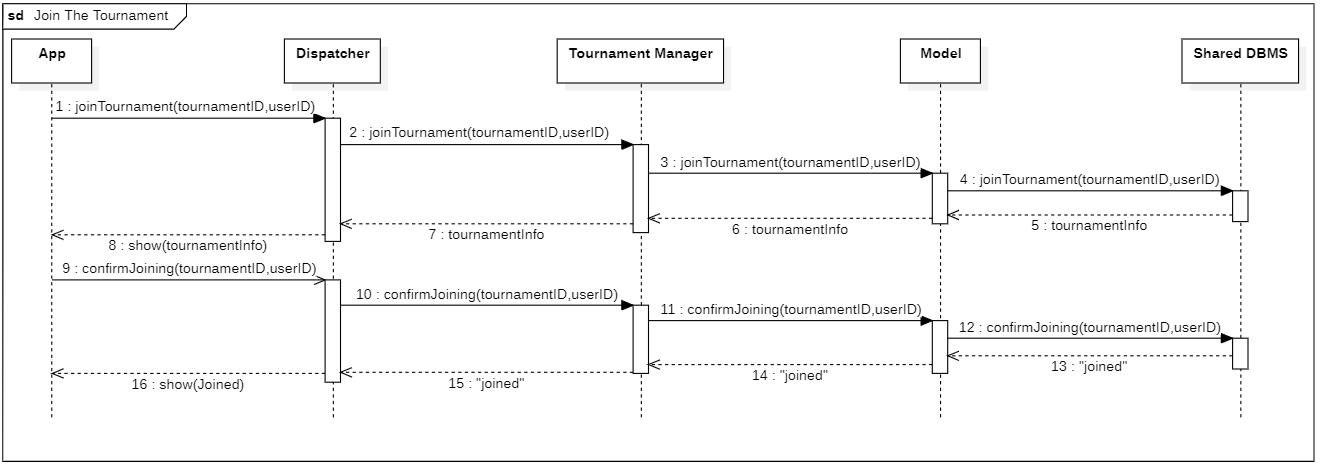
\includegraphics[width=\linewidth]{UC6.png}
\end{figure}

\begin{figure}[H]
  \centering
  \textbf{[UC7] Badge Creation} \\
  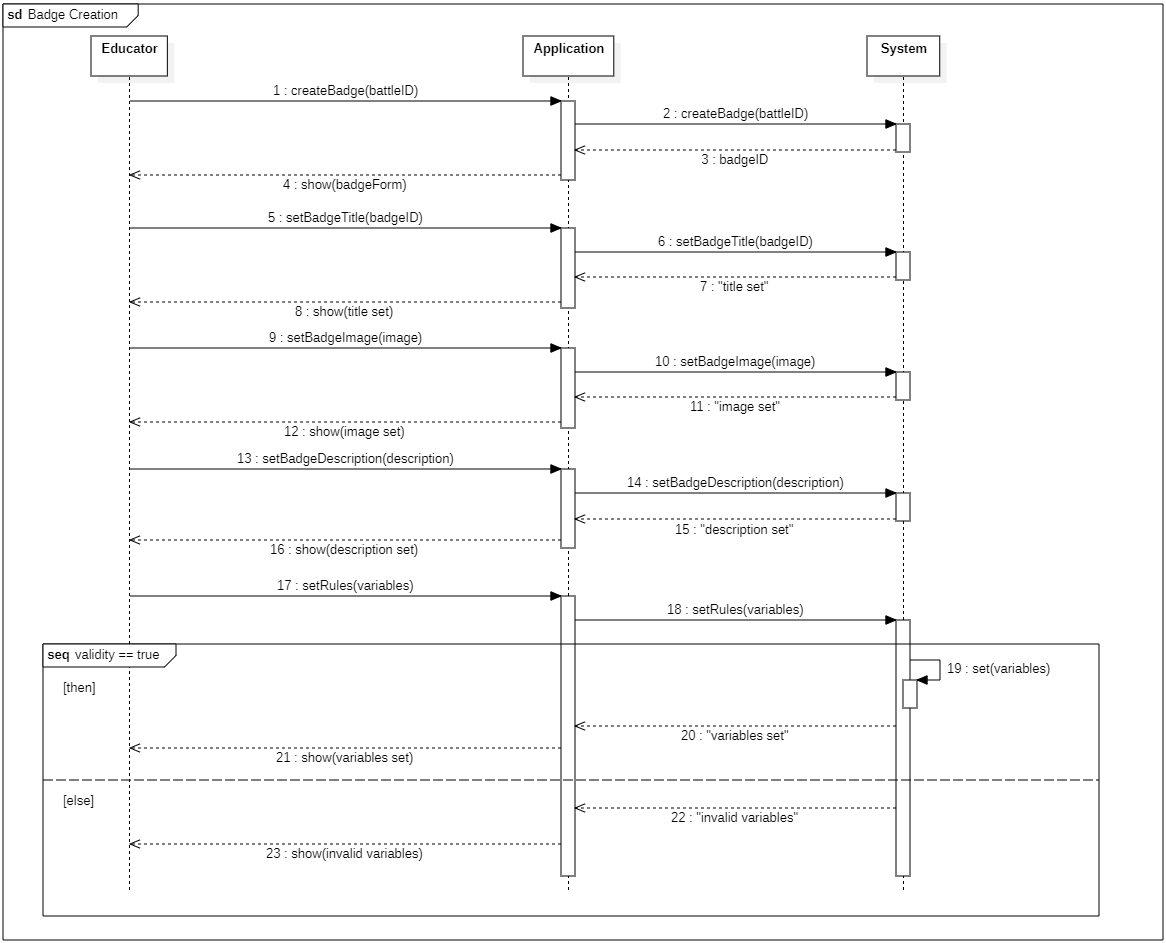
\includegraphics[width=\linewidth]{UC7.png}
\end{figure}

\begin{figure}[H]
  \centering
  \textbf{[UC8] Assigning A Badge} \\
  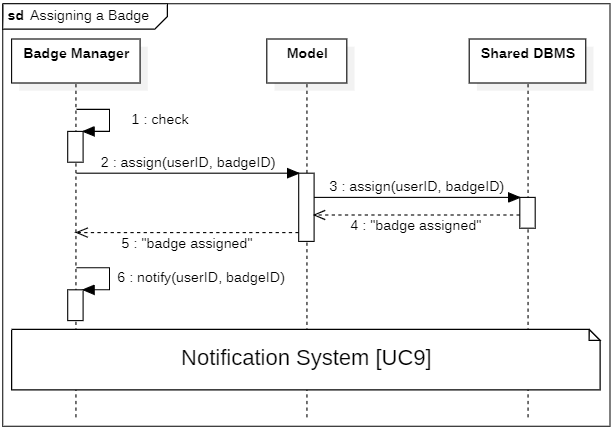
\includegraphics[width=\linewidth]{UC8.png}
\end{figure}

\begin{figure}[H]
  \centering
  \textbf{[UC9] Notification System} \\
  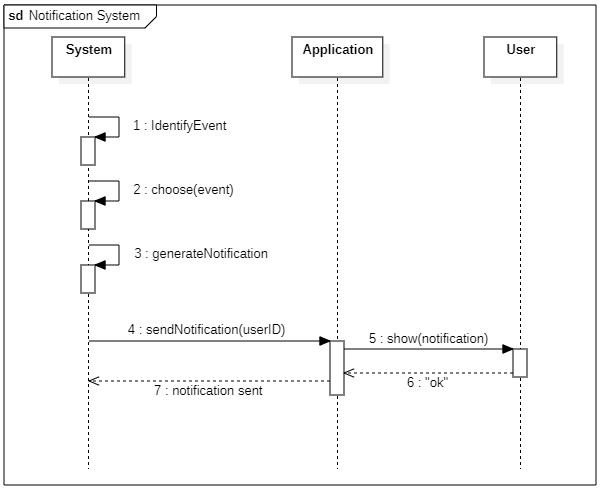
\includegraphics[width=\linewidth]{UC9.png}
\end{figure}

\begin{figure}[H]
  \centering
  \textbf{[UC10] Automated Evaluation} \\
  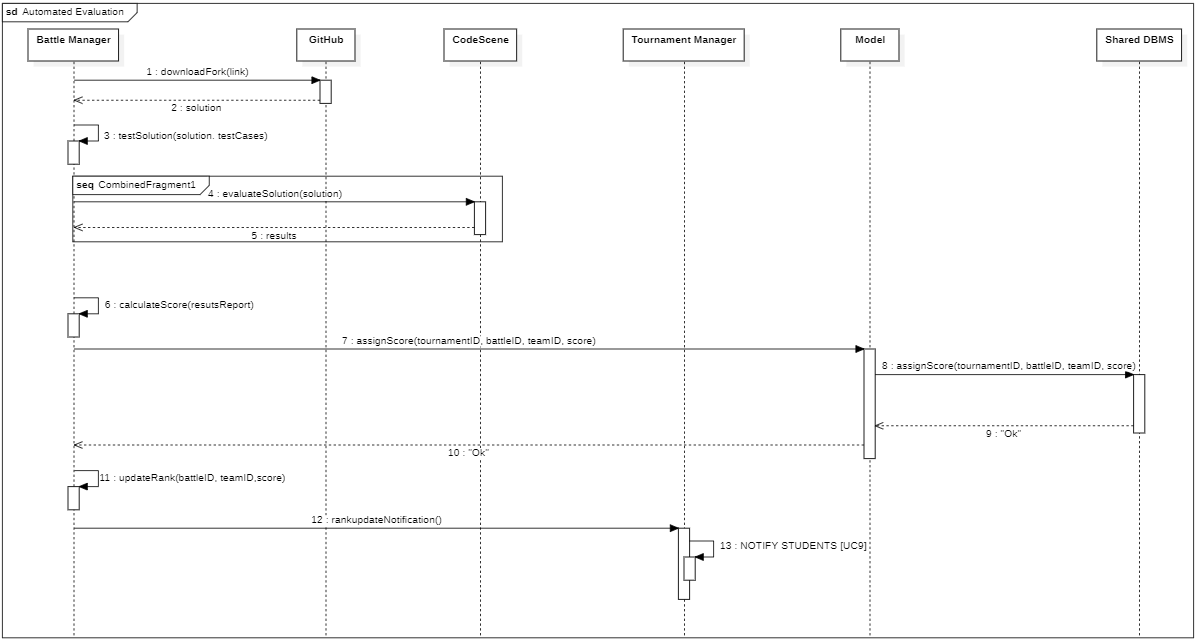
\includegraphics[width=\linewidth]{UC10.png}
\end{figure}

\begin{figure}[H]
  \centering
  \textbf{[UC11] Manual Evaluation} \\
  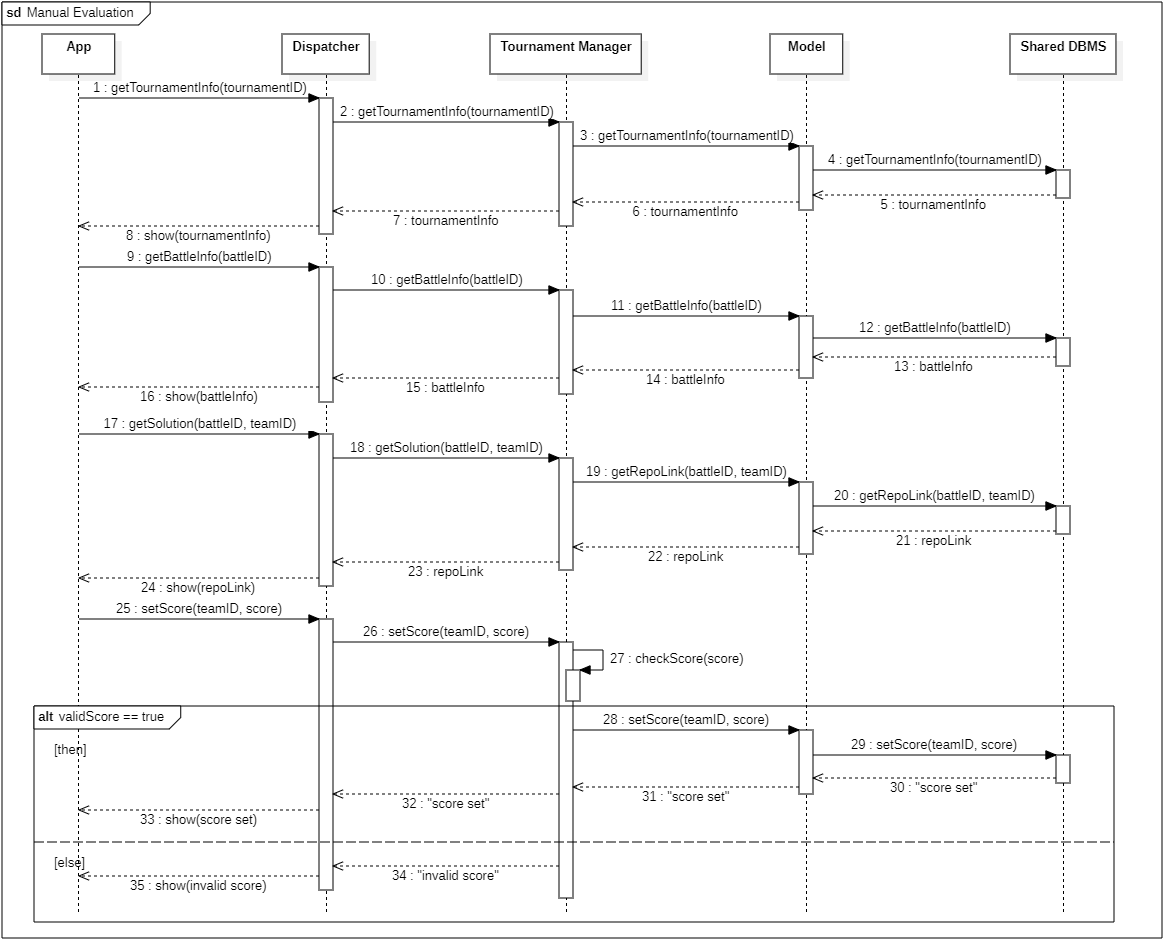
\includegraphics[width=\linewidth]{UC11.png}
\end{figure}

\begin{figure}[H]
  \centering
  \textbf{[UC12] Fork Creation} \\
  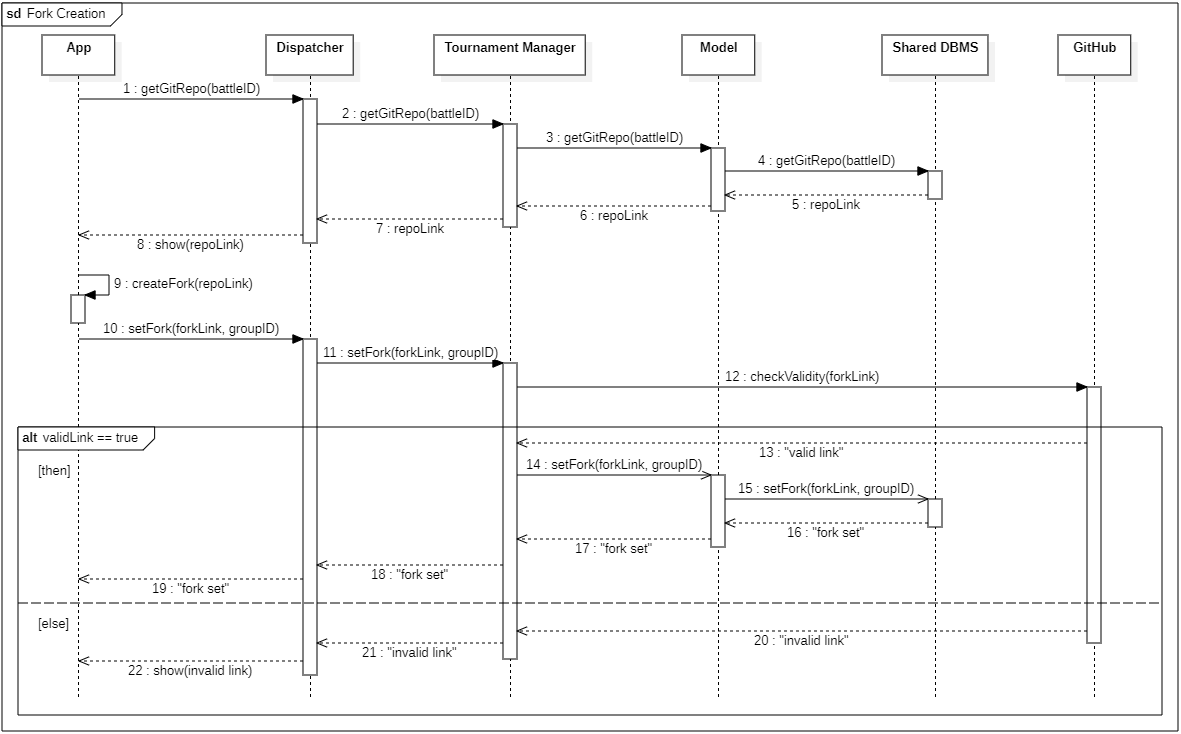
\includegraphics[width=\linewidth]{UC12.png}
\end{figure}

\begin{figure}[H]
    \centering
    \textbf{[UC13] Close Tournament} \\
    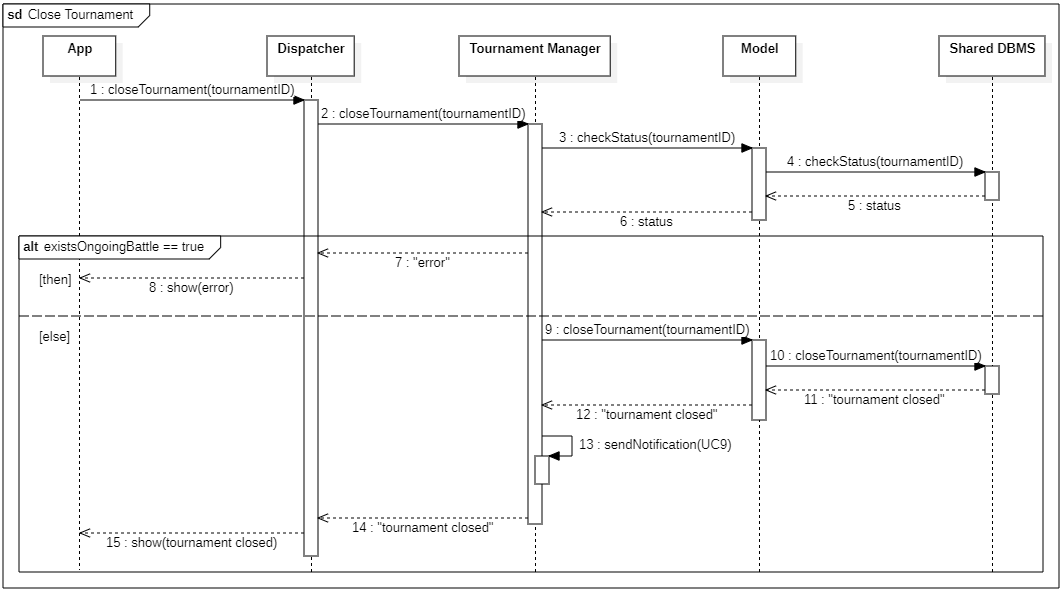
\includegraphics[width=\linewidth]{UC13.png} 
\end{figure}

\begin{figure}[H]
    \centering
    \textbf{[UC14] Visit Profile} \\
    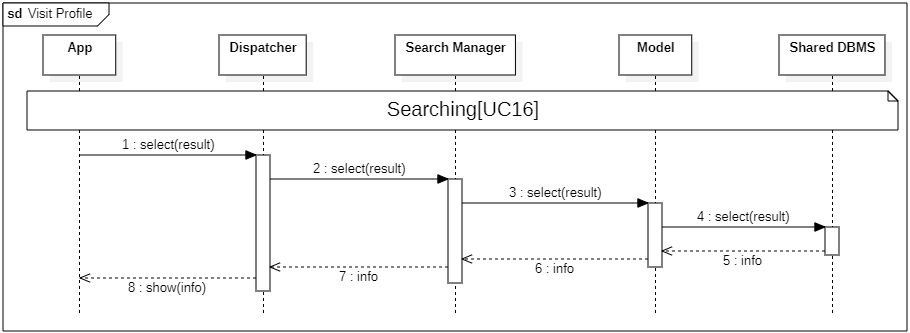
\includegraphics[width=\linewidth]{UC14.png} 
\end{figure}

\begin{figure}[H]
    \centering
    \textbf{[UC15] Joining Invitation} \\
    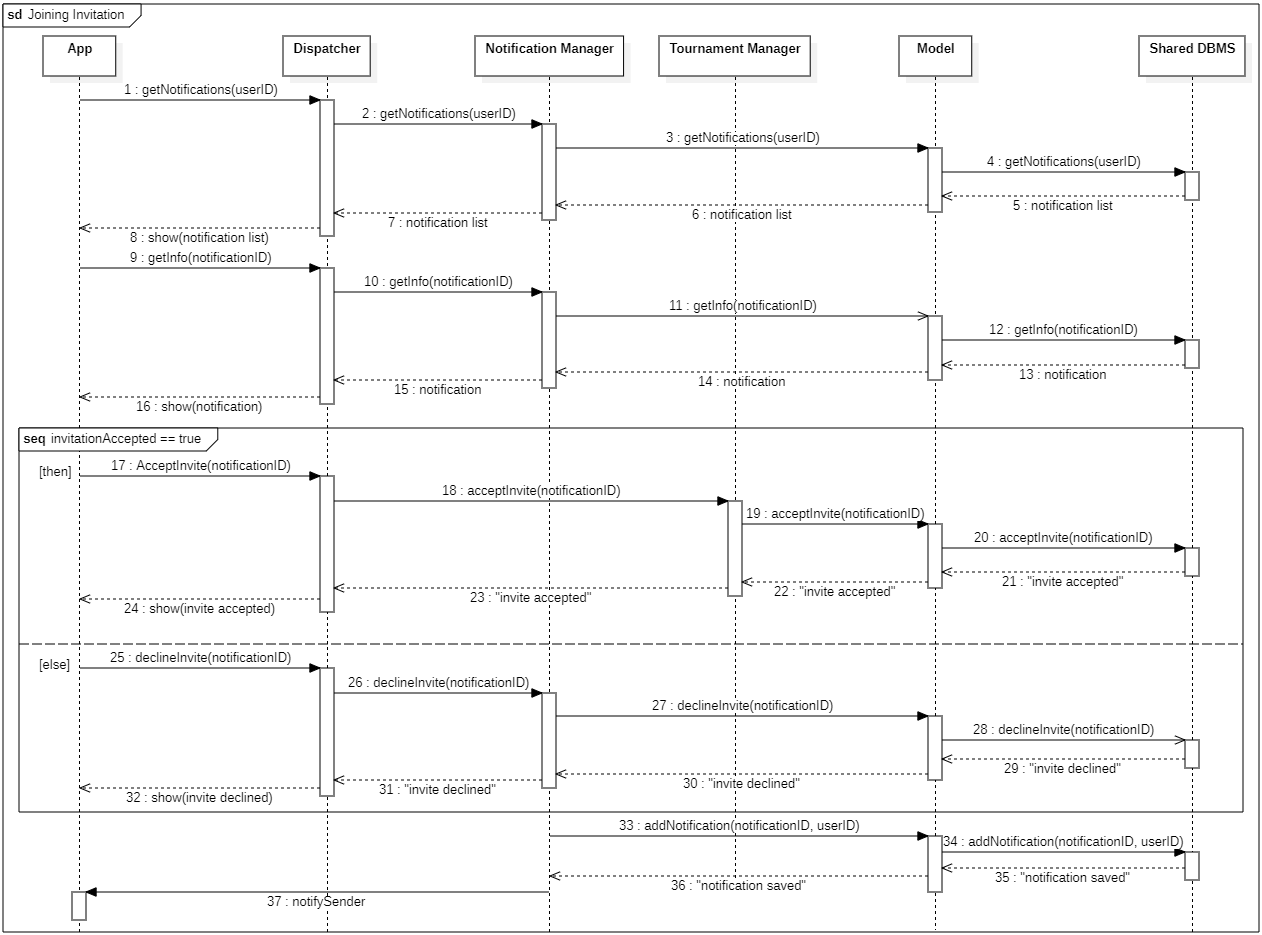
\includegraphics[width=\linewidth]{UC15.png} 
\end{figure}

\begin{figure}[H]
    \centering
    \textbf{[UC16] Searching} \\
    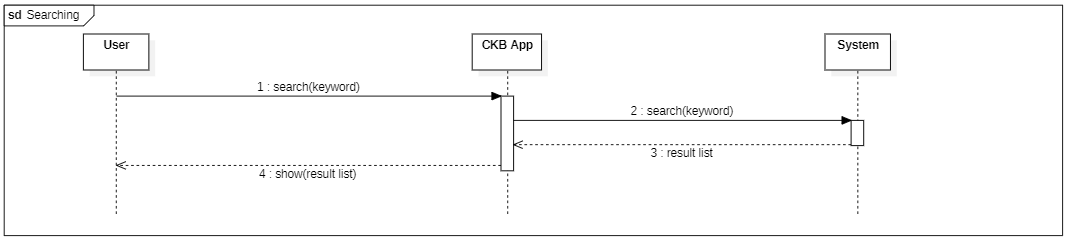
\includegraphics[width=\linewidth]{UC16.png} 
\end{figure}
\newpage
\subsubsection{Requirements Mapping}

\begin{table}[H]
\begin{adjustwidth}{-1in}{-1in}
 \renewcommand{\arraystretch}{1.5}
    \begin{tabular}{|p{9.5cm}|p{9.5cm}|}
        \hline
        \multicolumn{2}{|c|}{\textbf{[G1] EDUCATORS AND STUDENTS CAN SUBSCRIBE TO THE APPLICATION CREATING}} \\
        \multicolumn{2}{|c|}{\textbf{THEIR PERSONAL ACCOUNT}}\\
        \hline
        \begin{itemize}[label={}, left=0pt, align=left, itemsep=5pt]
            \item \textbf{[FR1]} The system allows Users (Students and Educators) to sign up.
            \item \textbf{[FR2]} The system allows Users (Students and Educators) to login.
        \end{itemize} &
        \begin{itemize} [label={}, left=0pt, align=left, itemsep=5pt]
            \item \textbf{[D1]} User must have an internet connection. 
            \item \textbf{[D4]} Connection between systems must be reliable.
        \end{itemize} \\
        \hline
    \end{tabular}
\end{adjustwidth}
\end{table}

\begin{table}[H]
\begin{adjustwidth}{-1in}{-1in}
 \renewcommand{\arraystretch}{1.5}
    \begin{tabular}{|p{9.5cm}|p{9.5cm}|}
        \hline
        \multicolumn{2}{|c|}{\textbf{[G2] EDUCATORS CREATE TOURNAMENTS IN WHICH STUDENTS CAN COMPETE}} \\
        \hline
        \begin{itemize}[label={}, left=0pt, align=left, itemsep=5pt]
            \item \textbf{[FR3]} The system allows Educators to create tournaments.
            \item \textbf{[FR4]} The system allows Educators to set a deadline for subscribing to the tournament.
            \item \textbf{[FR5]} The System allows Educators to set a list of programming languages that will be used in the tournament.
            \item \textbf{[FR6]} The system allows Educators to invite other Educators as collaborators for a tournament
            \item \textbf{[FR7]} The system allows Educators to set the number of battles in a tournament.
            \item \textbf{[FR22]} The system allows Educators to see the list of the active tournaments they have created.
        \end{itemize} &
        \begin{itemize}[label={}, left=0pt, align=left, itemsep=5pt]
            \item \textbf{[D1]} User must have an internet connection.
            \item \textbf{[D4]} Connection between systems must be reliable.
        \end{itemize} \\
        \hline
    \end{tabular}
\end{adjustwidth}
\end{table}

\begin{table}[H]
\begin{adjustwidth}{-1in}{-1in}
 \renewcommand{\arraystretch}{1.5}
    \begin{tabular}{|p{9.5cm}|p{9.5cm}|}
        \hline
        \multicolumn{2}{|c|}{\textbf{[G3] STUDENTS SUBSCRIBE TO THE TOURNAMENTS}} \\
        \hline
        \begin{itemize}[label={}, left=0pt, align=left, itemsep=5pt]
            \item \textbf{[FR18]} The system allows Students to join a tournament.
            \item \textbf{[FR23]} The system allows Students to see the list of the active tournaments they have joined.
        \end{itemize} &
        \begin{itemize}[label={}, left=0pt, align=left, itemsep=5pt]
            \item \textbf{[D1]} User must have an internet connection.
            \item \textbf{[D4]} Connection between systems must be reliable.
        \end{itemize} \\
        \hline
    \end{tabular}
\end{adjustwidth}
\end{table}

\begin{table}[H]
\begin{adjustwidth}{-1in}{-1in}
 \renewcommand{\arraystretch}{1.5}
    \begin{tabular}{|p{9.5cm}|p{9.5cm}|}
        \hline
        \multicolumn{2}{|c|}{\textbf{[G4] EDUCATORS CREATE BATTLES IN THE CONTEXT OF A TOURNAMENT,}} \\
        \multicolumn{2}{|c|}{\textbf{CONSISTING IN CODING CHALLENGES FOR STUDENTS}} \\
        \hline
        \begin{itemize}[label={}, left=0pt, align=left, itemsep=5pt]
            \item \textbf{[FR8]} The system allows Educators to create battles.
            \item \textbf{[FR9]} The system allows Educators to set a deadline for the subscription to the battle.
            \item \textbf{[FR10]} The system allows Educators to set a deadline for the submission of the solutions to the battle.
            \item \textbf{[FR11]} The System allows educators to choose which of the languages of the tournament will be used in each battle.
            \item \textbf{[FR12]} The System allows Educators to upload the files with the text of the problem and test cases for the battle
            \item \textbf{[FR13]} The system allows Educators to set the maximum number of students per team in a battle.
            \item \textbf{[FR14]} The system allows Educators to choose whether and when the scores will be assigned in a totally automatic way or also through manual verification by themselves
        \end{itemize} &
        \begin{itemize}[label={}, left=0pt, align=left, itemsep=5pt]
            \item \textbf{[D1]} User must have an internet connection.
            \item \textbf{[D4]} Connection between systems must be reliable.
            \item \textbf{[D5]} Test cases provided by educators must be correct.
            \item \textbf{[D6]} GitHub works as expected.
        \end{itemize} \\
        \hline
    \end{tabular}
\end{adjustwidth}
\end{table}

\begin{table}[H]
\begin{adjustwidth}{-1in}{-1in}
 \renewcommand{\arraystretch}{1.5}
    \begin{tabular}{|p{9.5cm}|p{9.5cm}|}
        \hline
        \multicolumn{2}{|c|}{\textbf{[G5] STUDENTS COMPETE, IN TEAMS OR ON THEIR OWN, IN MANY BATTLES,}} \\
        \multicolumn{2}{|c|}{\textbf{THE RESULTS OF WHICH WILL DETERMINE THE FINAL RANK OF THE TOURNAMENT}} \\
        \hline
        \begin{itemize}[label={}, left=0pt, align=left, itemsep=5pt]
            \item \textbf{[FR19]} The system allows Students to invite other students to form teams for a battle
            \item \textbf{[FR20]} The system allows Students to join a battle.
            \item \textbf{[FR21]} The system allows Students to know about the provisional scores of all students, updated for every solution submitted, for the duration of a battle.
        \end{itemize} &
        \begin{itemize}[label={}, left=0pt, align=left, itemsep=5pt]
            \item \textbf{[D1]} User must have an internet connection.
            \item \textbf{[D2]} User must have a GitHub account.
            \item \textbf{[D3]} User must know how to use GitHub in the proper way (push, pull, branch, etc.).
            \item \textbf{[D4]} Connection between systems must be reliable.
            \item \textbf{[D5]} Test cases provided by educators must be correct.
            \item \textbf{[D6]} GitHub works as expected.
            \item \textbf{[D7]} The static Analysis tool works reliably.
        \end{itemize} \\
        \hline
    \end{tabular}
\end{adjustwidth}
\end{table}

\begin{table}[H]
\begin{adjustwidth}{-1in}{-1in}
 \renewcommand{\arraystretch}{1.5}
    \begin{tabular}{|p{9.5cm}|p{9.5cm}|}
        \hline
        \multicolumn{2}{|c|}{\textbf{[G6] EDUCATORS CREATE BADGES AND DEFINE REQUIREMENTS TO ACHIEVE THEM}} \\
        \hline
        \begin{itemize}[label={}, left=0pt, align=left, itemsep=5pt]
            \item \textbf{[FR15]} The system allows Educators to create badges for a specific tournament.
            \item \textbf{[FR16]} The system allows Educators to build the requirements for achieving a badge.
        \end{itemize} &
        \begin{itemize}[label={}, left=0pt, align=left, itemsep=5pt]
            \item \textbf{[D1]} User must have an internet connection.
            \item \textbf{[D4]} Connection between systems must be reliable.
        \end{itemize} \\
        \hline
    \end{tabular}
\end{adjustwidth}
\end{table}

\begin{table}[H]
\begin{adjustwidth}{-1in}{-1in}
 \renewcommand{\arraystretch}{1.5}
    \begin{tabular}{|p{9.5cm}|p{9.5cm}|}
        \hline
        \multicolumn{2}{|c|}{\textbf{[G7] STUDENTS CAN REACH ACHIEVEMENTS}} \\
        \multicolumn{2}{|c|}{\textbf{THAT PERMIT THEM TO GAIN BADGES FOR THEIR ACCOUNT}} \\
        \hline
        \begin{itemize}[label={}, left=0pt, align=left, itemsep=5pt]
            \item \textbf{[FR17]} The system allows Students to see what are the active badges in a tournament and what they have to do to achieve them.
        \end{itemize} &
        \begin{itemize}[label={}, left=0pt, align=left, itemsep=5pt]
            \item \textbf{[D1]} User must have an internet connection.
            \item \textbf{[D4]} Connection between systems must be reliable.
        \end{itemize} \\
        \hline
    \end{tabular}
\end{adjustwidth}
\end{table}

\begin{table}[H]
\begin{adjustwidth}{-1in}{-1in}
 \renewcommand{\arraystretch}{1.5}
    \begin{tabular}{|p{9.5cm}|p{9.5cm}|}
        \hline
        \multicolumn{2}{|c|}{\textbf{[G8] USERS CAN VISIT THE ACCOUNT OF EACH OTHER AS PART OF A COMMUNITY,}} \\
        \multicolumn{2}{|c|}{\textbf{THEIR STATS AND ACHIEVED BADGES ARE PUBLIC.}} \\
        \hline
        \begin{itemize}[label={}, left=0pt, align=left, itemsep=5pt]
            \item \textbf{[FR24]} The system allows Users to see the stats of any other account registered in the system.
            \item \textbf{[FR25]} The system allows Users to search for other accounts or tournaments on the search bar.
        \end{itemize} &
        \begin{itemize}[label={}, left=0pt, align=left, itemsep=5pt]
            \item \textbf{[D1]} User must have an internet connection.
            \item \textbf{[D4]} Connection between systems must be reliable.
        \end{itemize} \\
        \hline
    \end{tabular}
\end{adjustwidth}
\end{table}

\newpage

\subsection{Performance Requirements}
The CKB app is designed to ensure optimal performance, capable of serving a large number of users. Users can expect a swift system response, typically within a couple of seconds, assuming a stable internet connection. In instances of slower internet connections, response times may vary due to external factors beyond the system's control. The app is equipped to detect and handle such conditions to provide the best possible user experience.

\subsection{Design Constraints}

\subsubsection{Standards compliance}
Regarding data privacy, the KCB project is committed to compliance with the General Data Protection Regulation (GDPR). The GDPR is a comprehensive regulation within EU law designed to protect and ensure the privacy of individuals within the European Union (EU) and the European Economic Area (EEA) concerning the processing of personal data. \\
In addition to data privacy regulations, the system also adheres to international standards concerning the use and representation of date and time. This ensures consistency and compatibility in handling temporal information, aligning the system with global norms.

\subsubsection{Hardware limitations}
The following system requirements must be met for CKB to function properly:
\begin{itemize}
    \item For the mobile app, an internet connection(mobile data or Wi-Fi) and an updated OS(iOS or Android) are required. 
    \item For the web app, an internet connection(mobile data or Wi-Fi) and an updated web browser is required.
\end{itemize}

\subsubsection{Any other constraint}
Since the system is designed to allow users to participate in coding battles, the system should not be too simple nor too detailed, allowing users to easily navigate through the various sections of the app.

\subsection{Software System Attributes}

\subsubsection{Reliability}
The system should achieve an uptime of at least 99.9\%, implement mechanisms for graceful degradation during system failures, and ensure consistent and reliable storage of user data and kata progress.

\subsubsection{Availability}
The system should maintain a 24/7 availability, with advanced communication for scheduled maintenance.\\
Since this is not a critical system, a downtime period(for maintenance or disservice) is acceptable.

\subsubsection{Security}
Since it stores some personal information, the system should use secure channels for all user interactions, employing industry-standard encryption protocols and implementing robust user authentication and authorization mechanisms, furthermore, there should be conducted regular security audits and vulnerability assessments.

\subsubsection{Maintainability}
The system should adhere to industry coding standards and best practices for a maintainable codebase, maintain comprehensive documentation, including API references and system architecture, and support easy integration of new code katas with deployable updates and minimal downtime.

\subsubsection{Portability}
The application is required to be developed for two distinct platforms: iOS and Android devices. Additionally, the web application must be compatible with any operating system—such as Windows, Mac OS, Linux, and others—that supports a standard web browser.
\newpage
\section{Formal Analysis Using Alloy}
All the signatures defined for the Alloy modelization are listed below.
\subsection{Signatures}
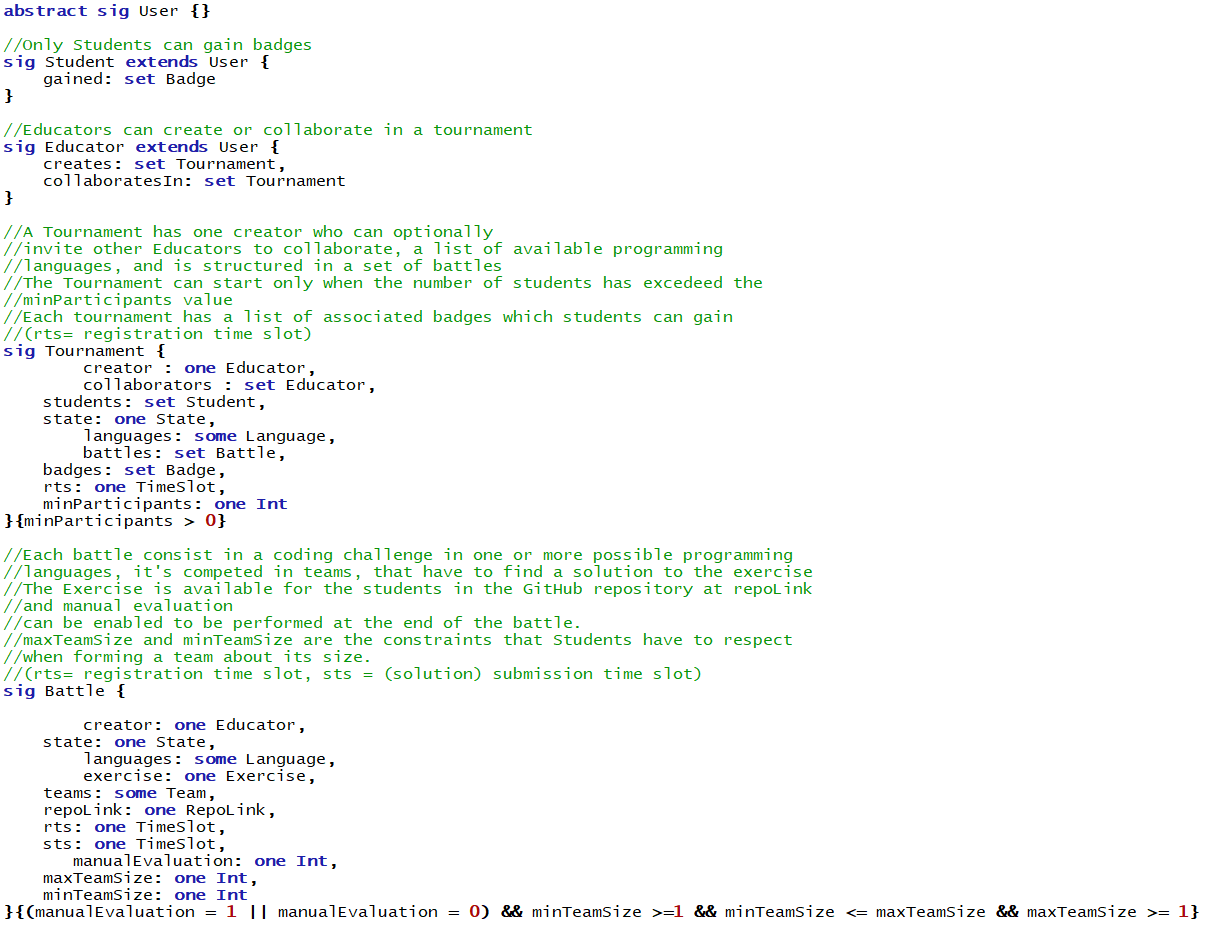
\includegraphics[width=\textwidth,height=\textheight,keepaspectratio]{Signatures1.png}
\newpage
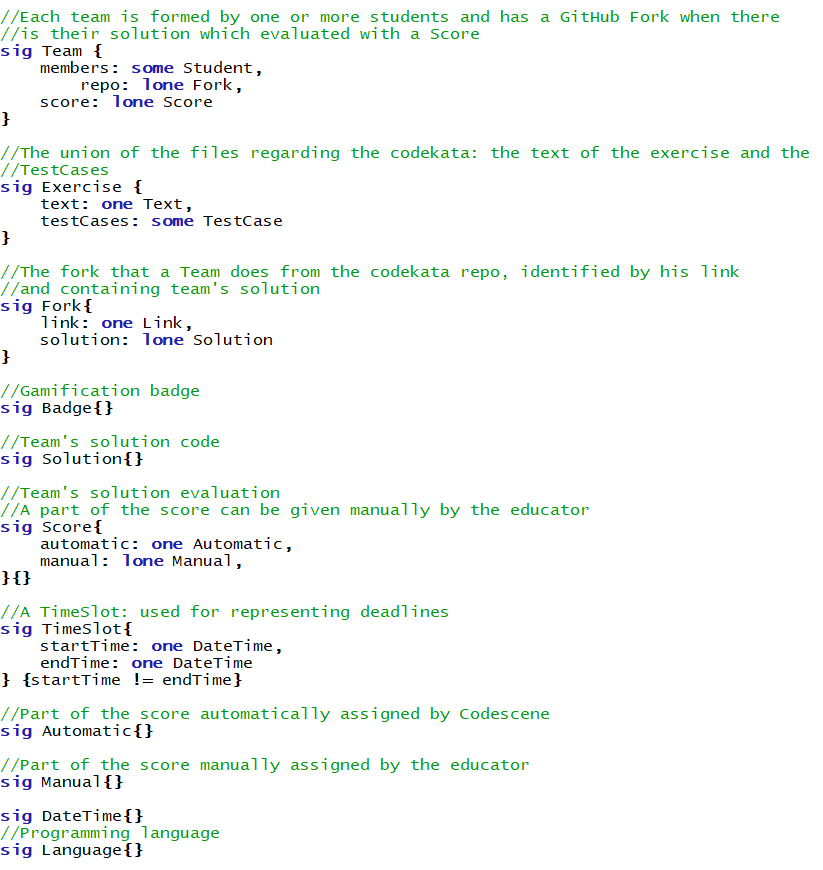
\includegraphics[width=\textwidth,height=\textheight,keepaspectratio]{Signatures2.png}
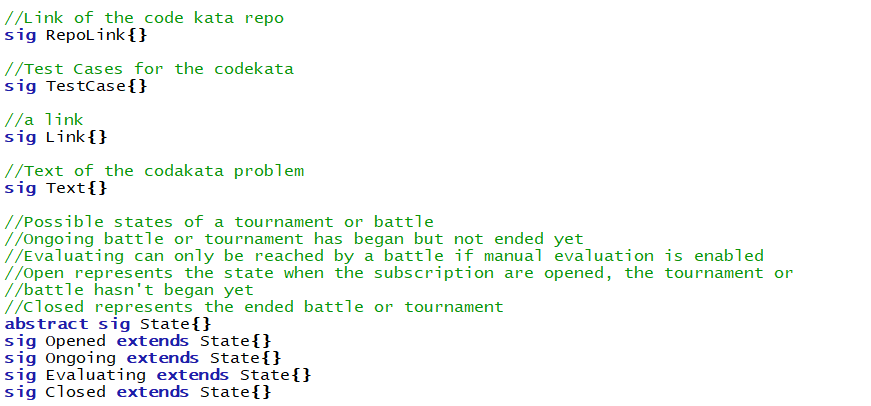
\includegraphics[width=\textwidth,height=\textheight,keepaspectratio]{Signatures3.png}
\newpage
\subsection{Facts}
The following facts are stated in Alloy, representing the requirements that must be held for the domain to remain consistent with the real world. \\
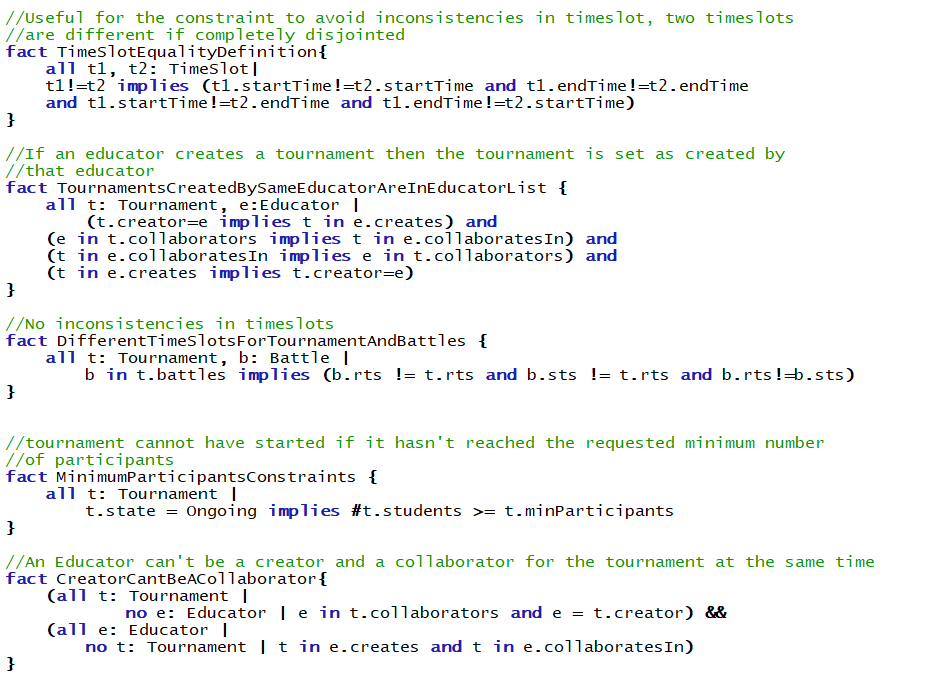
\includegraphics[width=\textwidth,height=\textheight,keepaspectratio]{Facts1.png}
\newpage
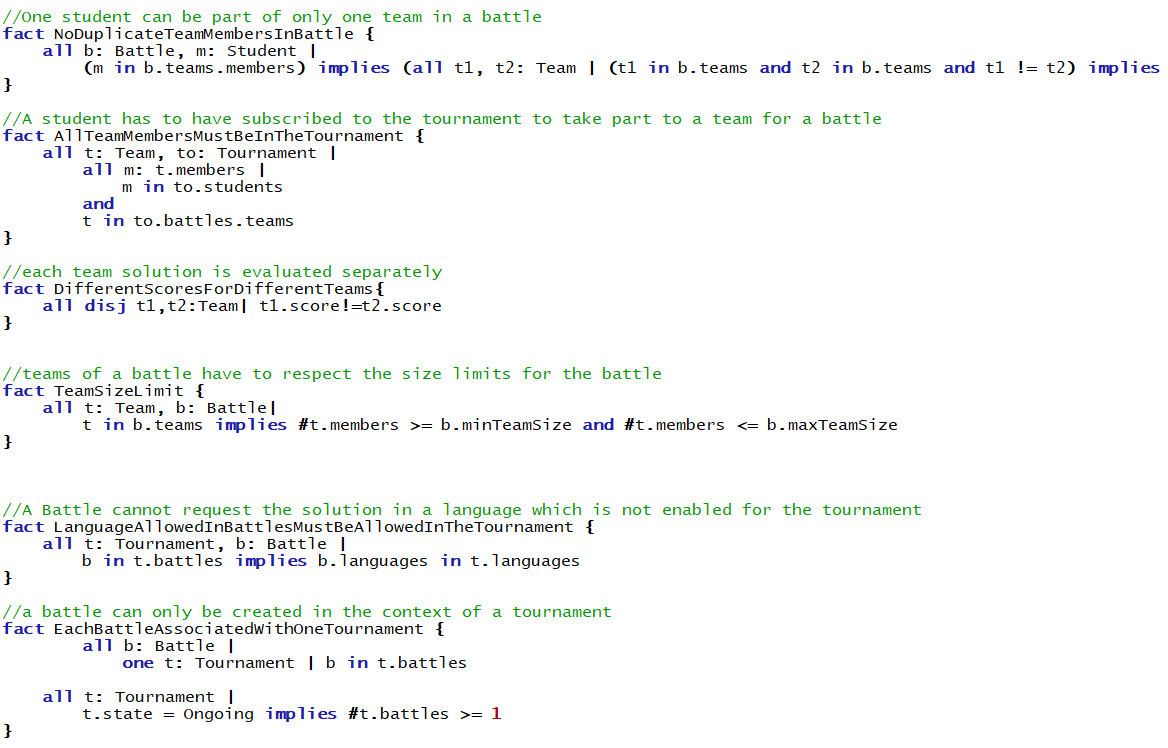
\includegraphics[width=\textwidth,height=\textheight,keepaspectratio]{Facts2.png}
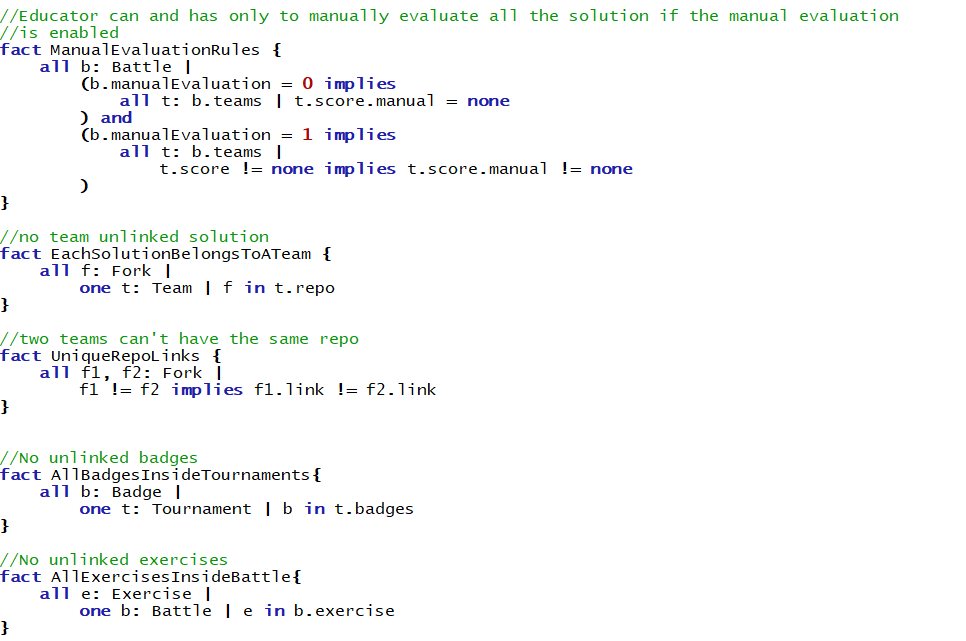
\includegraphics[width=\textwidth,height=\textheight,keepaspectratio]{Facts3.png}
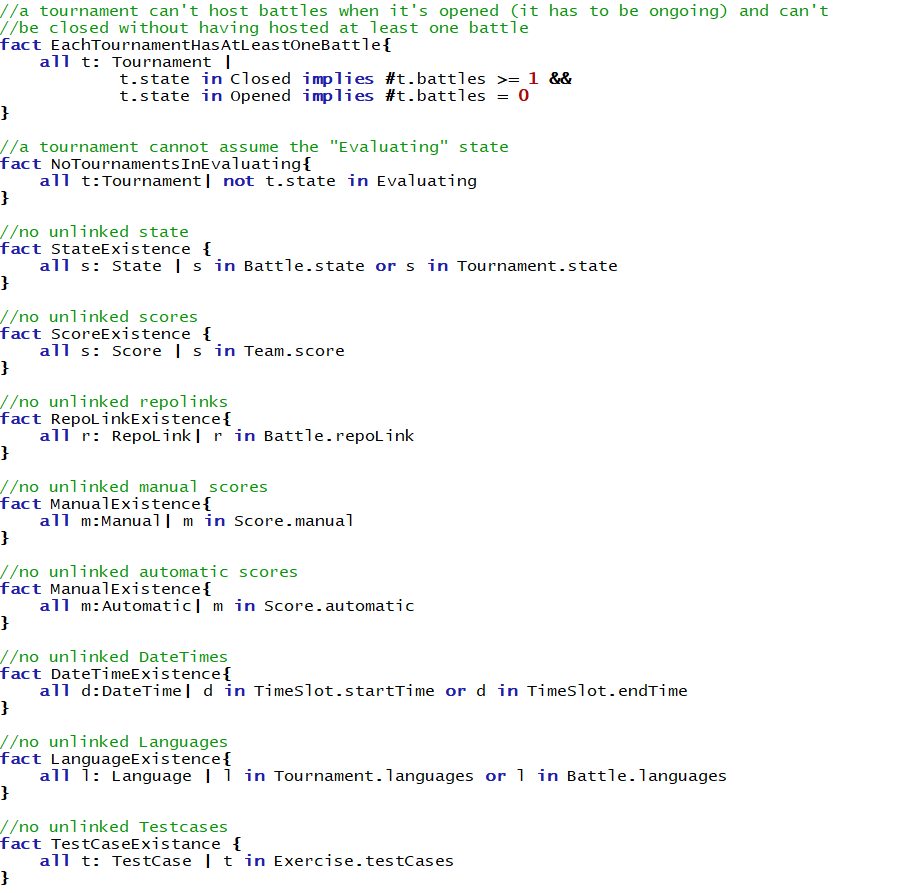
\includegraphics[width=\textwidth,height=\textheight,keepaspectratio]{Facts4.png}
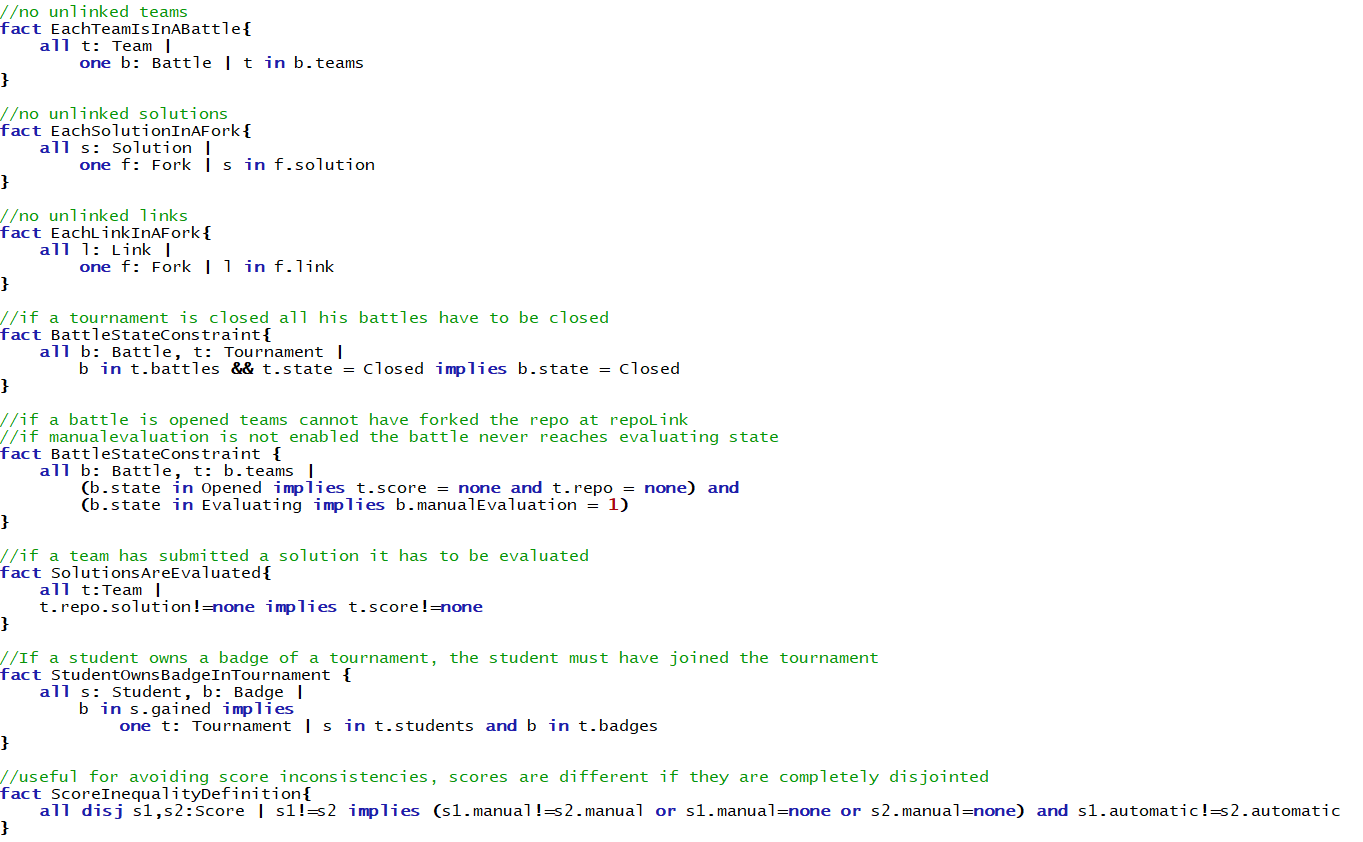
\includegraphics[width=\textwidth,height=\textheight,keepaspectratio]{Facts5.png}
\newpage
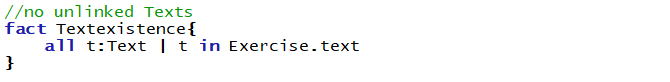
\includegraphics[width=\textwidth,height=\textheight,keepaspectratio]{Facts6.png}
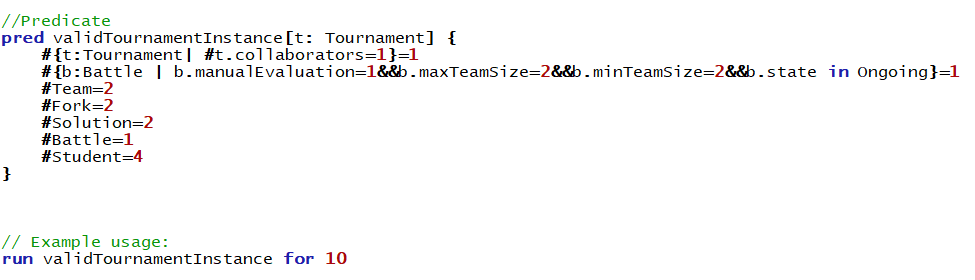
\includegraphics[width=\textwidth,height=\textheight,keepaspectratio]{Predicate.png}
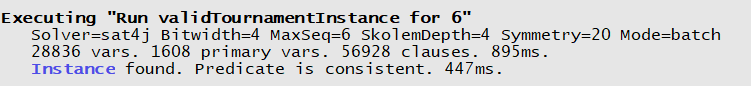
\includegraphics[width=\textwidth,height=\textheight,keepaspectratio]{Result.png}

\begin{figure}[H]
    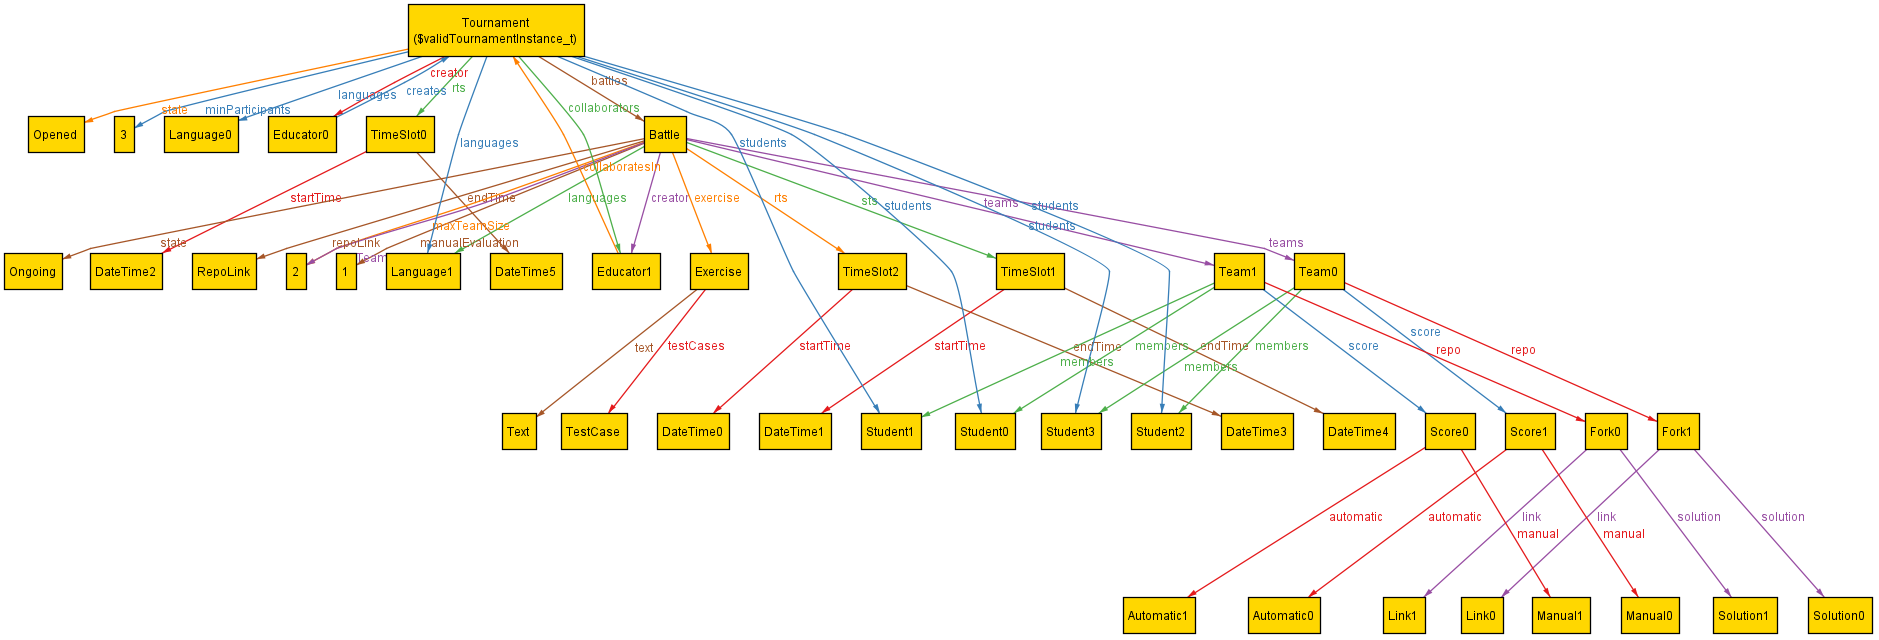
\includegraphics[width=\textwidth,height=\textheight,keepaspectratio]{AlloyModel.png}
    \caption{Metamodel showing the status of a tournament}
\end{figure}
\newpage

\section{Effort Spent}
\begin{center}
\textbf{Armando Fiorini} \\
\vspace{10px}
    \begin{tabularx}{0.8\textwidth} { 
  | >{\centering\arraybackslash}X 
  | >{\centering\arraybackslash}X | }
 \hline
 \textbf{Chapter} & \textbf{Hours Spent} \\
 \hline
 1 & 3  \\
 \hline
 2 & 10 \\
 \hline
 3 & 21 \\
 \hline
 4 & 18 \\
 \hline
\end{tabularx}

\vspace{10px}
\textbf{Samuele Motta} \\
\vspace{10px}
\begin{tabularx}{0.8\textwidth} { 
  | >{\centering\arraybackslash}X 
  | >{\centering\arraybackslash}X | }
 \hline
 \textbf{Chapter} & \textbf{Hours Spent} \\
 \hline
 1 & 4  \\
 \hline
 2 & 6 \\
 \hline
 3 & 20 \\
 \hline
 4 & 14 \\
 \hline
\end{tabularx}

\vspace{10px}
\textbf{Vajihe Gholami} \\
\vspace{10px}
\begin{tabularx}{0.8\textwidth} { 
  | >{\centering\arraybackslash}X 
  | >{\centering\arraybackslash}X | }
 \hline
 \textbf{Chapter} & \textbf{Hours Spent} \\
 \hline
 1 & 4  \\
 \hline
 2 & 11 \\
 \hline
 3 & 22 \\
 \hline
 4 & 10 \\
 \hline
\end{tabularx}

\end{center}

\section{References}
\begin{itemize}
    \item Diagrams made with StarUML
    \item Mockups made with: moqups.com
    \item Alloy models checked and ran with Alloy analyzer
\end{itemize}

\end{document}